\documentclass[twoside]{book}

% Packages required by doxygen
\usepackage{calc}
\usepackage{doxygen}
\usepackage{graphicx}
\usepackage[utf8]{inputenc}
\usepackage{makeidx}
\usepackage{multicol}
\usepackage{multirow}
\usepackage{textcomp}
\usepackage[table]{xcolor}

% Font selection
\usepackage[T1]{fontenc}
\usepackage{mathptmx}
\usepackage[scaled=.90]{helvet}
\usepackage{courier}
\usepackage{amssymb}
\usepackage{sectsty}
\renewcommand{\familydefault}{\sfdefault}
\allsectionsfont{%
  \fontseries{bc}\selectfont%
  \color{darkgray}%
}
\renewcommand{\DoxyLabelFont}{%
  \fontseries{bc}\selectfont%
  \color{darkgray}%
}

% Page & text layout
\usepackage{geometry}
\geometry{%
  a4paper,%
  top=2.5cm,%
  bottom=2.5cm,%
  left=2.5cm,%
  right=2.5cm%
}
\tolerance=750
\hfuzz=15pt
\hbadness=750
\setlength{\emergencystretch}{15pt}
\setlength{\parindent}{0cm}
\setlength{\parskip}{0.2cm}
\makeatletter
\renewcommand{\paragraph}{%
  \@startsection{paragraph}{4}{0ex}{-1.0ex}{1.0ex}{%
    \normalfont\normalsize\bfseries\SS@parafont%
  }%
}
\renewcommand{\subparagraph}{%
  \@startsection{subparagraph}{5}{0ex}{-1.0ex}{1.0ex}{%
    \normalfont\normalsize\bfseries\SS@subparafont%
  }%
}
\makeatother

% Headers & footers
\usepackage{fancyhdr}
\pagestyle{fancyplain}
\fancyhead[LE]{\fancyplain{}{\bfseries\thepage}}
\fancyhead[CE]{\fancyplain{}{}}
\fancyhead[RE]{\fancyplain{}{\bfseries\leftmark}}
\fancyhead[LO]{\fancyplain{}{\bfseries\rightmark}}
\fancyhead[CO]{\fancyplain{}{}}
\fancyhead[RO]{\fancyplain{}{\bfseries\thepage}}
\fancyfoot[LE]{\fancyplain{}{}}
\fancyfoot[CE]{\fancyplain{}{}}
\fancyfoot[RE]{\fancyplain{}{\bfseries\scriptsize Generated on Fri Oct 3 2014 23\-:13\-:26 for C\-P\-P\-Data\-Structure by Doxygen }}
\fancyfoot[LO]{\fancyplain{}{\bfseries\scriptsize Generated on Fri Oct 3 2014 23\-:13\-:26 for C\-P\-P\-Data\-Structure by Doxygen }}
\fancyfoot[CO]{\fancyplain{}{}}
\fancyfoot[RO]{\fancyplain{}{}}
\renewcommand{\footrulewidth}{0.4pt}
\renewcommand{\chaptermark}[1]{%
  \markboth{#1}{}%
}
\renewcommand{\sectionmark}[1]{%
  \markright{\thesection\ #1}%
}

% Indices & bibliography
\usepackage{natbib}
\usepackage[titles]{tocloft}
\setcounter{tocdepth}{3}
\setcounter{secnumdepth}{5}
\makeindex

% Hyperlinks (required, but should be loaded last)
\usepackage{ifpdf}
\ifpdf
  \usepackage[pdftex,pagebackref=true]{hyperref}
\else
  \usepackage[ps2pdf,pagebackref=true]{hyperref}
\fi
\hypersetup{%
  colorlinks=true,%
  linkcolor=blue,%
  citecolor=blue,%
  unicode%
}

% Custom commands
\newcommand{\clearemptydoublepage}{%
  \newpage{\pagestyle{empty}\cleardoublepage}%
}


%===== C O N T E N T S =====

\begin{document}

% Titlepage & ToC
\hypersetup{pageanchor=false}
\pagenumbering{roman}
\begin{titlepage}
\vspace*{7cm}
\begin{center}%
{\Large C\-P\-P\-Data\-Structure }\\
\vspace*{1cm}
{\large Generated by Doxygen 1.8.6}\\
\vspace*{0.5cm}
{\small Fri Oct 3 2014 23:13:26}\\
\end{center}
\end{titlepage}
\clearemptydoublepage
\tableofcontents
\clearemptydoublepage
\pagenumbering{arabic}
\hypersetup{pageanchor=true}

%--- Begin generated contents ---
\chapter{Project C\-P\-P\-Data\-Structure}
\label{md_README}
\hypertarget{md_README}{}
Prueba Changed 
\chapter{Hierarchical Index}
\section{Class Hierarchy}
This inheritance list is sorted roughly, but not completely, alphabetically\-:\begin{DoxyCompactList}
\item \contentsline{section}{Double\-Node$<$ E $>$}{\pageref{classDoubleNode}}{}
\item \contentsline{section}{I\-Iterator$<$ E $>$}{\pageref{classIIterator}}{}
\begin{DoxyCompactList}
\item \contentsline{section}{Simple\-Iterator$<$ E $>$}{\pageref{classSimpleIterator}}{}
\end{DoxyCompactList}
\item \contentsline{section}{I\-List$<$ E $>$}{\pageref{classIList}}{}
\begin{DoxyCompactList}
\item \contentsline{section}{Circular\-List$<$ E $>$}{\pageref{classCircularList}}{}
\item \contentsline{section}{Double\-Circular\-List$<$ E $>$}{\pageref{classDoubleCircularList}}{}
\item \contentsline{section}{Double\-List$<$ E $>$}{\pageref{classDoubleList}}{}
\item \contentsline{section}{List$<$ E $>$}{\pageref{classList}}{}
\end{DoxyCompactList}
\item \contentsline{section}{Node$<$ E $>$}{\pageref{classNode}}{}
\item \contentsline{section}{Queue$<$ E $>$}{\pageref{classQueue}}{}
\item \contentsline{section}{Stack$<$ E $>$}{\pageref{classStack}}{}
\end{DoxyCompactList}

\chapter{Class Index}
\section{Lista de clases}
Lista de las clases, estructuras, uniones e interfaces con una breve descripción\-:\begin{DoxyCompactList}
\item\contentsline{section}{\hyperlink{classBArray}{B\-Array$<$ E $>$} \\*Clase \hyperlink{classBArray}{B\-Array}, esta clase da soporte al arbol b volviendolo menos complejo, mas facil de leer y sin asignarle al arbol b tareas como agregar los datos en orden en el array }{\pageref{classBArray}}{}
\item\contentsline{section}{\hyperlink{classBinaryNode}{Binary\-Node$<$ E $>$} \\*Esta clase es el elemento sustancial para los arboles binarios, contiene datos y punteros a la derecha e izquierda para generar esa estructura de los arboles binarios }{\pageref{classBinaryNode}}{}
\item\contentsline{section}{\hyperlink{classBinaryTree}{Binary\-Tree$<$ E $>$} \\*Clase Arbol Binario. Esta clase representa a la estructura de datos arbol binario, valga la rendondancia. Esta estructura de datos puede insertar, eliminar y buscar los datos relacionados con esta la misma. Usa platillas para almacenar diversos datos. Usa los operadores de comparacion como $<$, $>$, ==, $>$=, $<$= y != }{\pageref{classBinaryTree}}{}
\item\contentsline{section}{\hyperlink{classBNode}{B\-Node$<$ V\-A\-L\-U\-E $>$} }{\pageref{classBNode}}{}
\item\contentsline{section}{\hyperlink{classBTree}{B\-Tree$<$ K $>$} }{\pageref{classBTree}}{}
\item\contentsline{section}{\hyperlink{classCircularList}{Circular\-List$<$ E $>$} \\*Esta clase es una estructura de datos especificamente una lista enlazada circular simple que puede contener cualquier tipo de dato solamente definiciendolo mediante el template de esta clase. se puede agregar y borrar el dato }{\pageref{classCircularList}}{}
\item\contentsline{section}{\hyperlink{classCPPDataStructure}{C\-P\-P\-Data\-Structure} }{\pageref{classCPPDataStructure}}{}
\item\contentsline{section}{\hyperlink{classDoubleCircularList}{Double\-Circular\-List$<$ E $>$} \\*Esta clase es una estructura de datos especificamente una lista doblemente enlazada circular que puede contener cualquier tipo de dato solamente definiciendolo mediante el template de esta clase. se puede agregar y borrar el dato }{\pageref{classDoubleCircularList}}{}
\item\contentsline{section}{\hyperlink{classDoubleIterator}{Double\-Iterator$<$ E $>$} \\*Esta clase es un iterador de las listas doblemente enlazadas, ademas la actualizacion de la lista N\-O actualiza el iterador, por lo que el iterador es momentaneo. Es similar a una fotografia de una lista que no ha sido alterada si la lista se altera usando un iterador puede que el iterador falle. Por lo que es recomendable que la lista no se actualice mientras se usa un iterador }{\pageref{classDoubleIterator}}{}
\item\contentsline{section}{\hyperlink{classDoubleList}{Double\-List$<$ E $>$} \\*Esta clase es una estructura de datos especificamente una lista doblemente enlazada que puede contener cualquier tipo de dato solamente definiciendolo mediante el template de esta clase. se puede agregar y borrar el dato }{\pageref{classDoubleList}}{}
\item\contentsline{section}{\hyperlink{classDoubleListAdapter}{Double\-List\-Adapter$<$ E $>$} }{\pageref{classDoubleListAdapter}}{}
\item\contentsline{section}{\hyperlink{classDoubleNode}{Double\-Node$<$ E $>$} \\*Es la parte elemental de una lista que sea doublemente enlazada }{\pageref{classDoubleNode}}{}
\item\contentsline{section}{\hyperlink{classIIterator}{I\-Iterator$<$ E $>$} \\*Es una interfaz para los iteradores hijos de este }{\pageref{classIIterator}}{}
\item\contentsline{section}{\hyperlink{classIList}{I\-List$<$ E $>$} \\*Es la interfaz de las listas }{\pageref{classIList}}{}
\item\contentsline{section}{\hyperlink{classInverseIterator}{Inverse\-Iterator$<$ E $>$} \\*Esta clase es un iterador de las listas doblemente enlazadas, ademas la actualizacion de la lista N\-O actualiza el iterador, por lo que el iterador es momentaneo. Es similar a una fotografia de una lista que no ha sido alterada si la lista se altera usando un iterador puede que el iterador falle. Por lo que es recomendable que la lista no se actualice mientras se usa un iterador. Ademas de que este iterador recorre la lista desde el dato final hasta el dato inicial }{\pageref{classInverseIterator}}{}
\item\contentsline{section}{\hyperlink{classIOrdinateList}{I\-Ordinate\-List$<$ E $>$} }{\pageref{classIOrdinateList}}{}
\item\contentsline{section}{\hyperlink{classList}{List$<$ E $>$} \\*Esta clase es una estructura de datos especificamente una lista enlazada simple que puede contener cualquier tipo de dato solamente definiciendolo mediante el template de esta clase. se puede agregar y borrar el dato }{\pageref{classList}}{}
\item\contentsline{section}{\hyperlink{classNode}{Node$<$ E $>$} \\*Es la parte elemental de una lista simple }{\pageref{classNode}}{}
\item\contentsline{section}{\hyperlink{classQueue}{Queue$<$ E $>$} }{\pageref{classQueue}}{}
\item\contentsline{section}{\hyperlink{classSimpleIterator}{Simple\-Iterator$<$ E $>$} \\*Esta clase es un iterador de las listas simples, ademas la actualizacion de la lista N\-O actualiza el iterador, por lo que el iterador es momentaneo. Es similar a una fotografia de una lista que no ha sido alterada si la lista se altera usando un iterador puede que el iterador falle. Por lo que es recomendable que la lista no se actualice mientras se usa un iterador }{\pageref{classSimpleIterator}}{}
\item\contentsline{section}{\hyperlink{classSimpleListAdapter}{Simple\-List\-Adapter$<$ E $>$} }{\pageref{classSimpleListAdapter}}{}
\item\contentsline{section}{\hyperlink{classStack}{Stack$<$ E $>$} }{\pageref{classStack}}{}
\end{DoxyCompactList}

\chapter{Class Documentation}
\hypertarget{classCircularList}{\section{Referencia de la plantilla de la Clase Circular\-List$<$ E $>$}
\label{classCircularList}\index{Circular\-List$<$ E $>$@{Circular\-List$<$ E $>$}}
}


Esta clase es una estructura de datos especificamente una lista enlazada circular simple que puede contener cualquier tipo de dato solamente definiciendolo mediante el template de esta clase. se puede agregar y borrar el dato.  




{\ttfamily \#include $<$Circular\-List.\-h$>$}



Herencias \hyperlink{classIList}{I\-List$<$ E $>$}.

\subsection*{Métodos públicos}
\begin{DoxyCompactItemize}
\item 
\hypertarget{classCircularList_aad23571a808ede6fc0432dca645ab2ca}{\hyperlink{classCircularList_aad23571a808ede6fc0432dca645ab2ca}{Circular\-List} ()}\label{classCircularList_aad23571a808ede6fc0432dca645ab2ca}

\begin{DoxyCompactList}\small\item\em \hyperlink{classCircularList}{Circular\-List}. Es el constructor de la lista circular simple. \end{DoxyCompactList}\item 
void \hyperlink{classCircularList_a6de0a0af406c738b95b0a6d898b69f8e}{addi} (E)
\begin{DoxyCompactList}\small\item\em Agrega un elemento al principio de la lista. \end{DoxyCompactList}\item 
void \hyperlink{classCircularList_a892b493309f36fb083fdd257388cfa36}{add} (E)
\begin{DoxyCompactList}\small\item\em Agregar un elemento al final de la lista. \end{DoxyCompactList}\item 
bool \hyperlink{classCircularList_af184d3ac2e3bba683a44a6cc19392b12}{add} (E, int)
\begin{DoxyCompactList}\small\item\em Agrega el elemento en el indice indicado. Si el indice es incorrecto no se agrega el elemento. \end{DoxyCompactList}\item 
bool \hyperlink{classCircularList_a4a6acfd818a0ae9055957ec80258c60a}{remove} (int)
\begin{DoxyCompactList}\small\item\em Remueve el dato en la posicion indicada por el parametro, en caso que el indice indicado sea incorrecto, osea que sea menor que cero o mayor o igual que el largo de la lista no alterara la lista. \end{DoxyCompactList}\item 
void \hyperlink{classCircularList_aa54489e11ad76bf929f92b1dce97a3a3}{set} (int, E)
\begin{DoxyCompactList}\small\item\em Setea el valor del dato que se encuentre en el indice citado con un nuevo valor. \end{DoxyCompactList}\item 
E \hyperlink{classCircularList_ad6783339c7ff05841fc62f74f809644d}{get} (int)
\begin{DoxyCompactList}\small\item\em Obtiene un dato el la posicion indicada. En caso que el indice indicado sea incorrecto, osea que sea menor que cero o mayor o igual que el largo de la lista arrojara un error pues el dato esta fuera de los limites de la lista. \end{DoxyCompactList}\item 
\hyperlink{classIIterator}{I\-Iterator}$<$ E $>$ $\ast$ \hyperlink{classCircularList_a43e6cf1632001b3f409c6ce531529c6e}{get\-Iterator} ()
\begin{DoxyCompactList}\small\item\em Obtiene una instancia de un nuevo iterador de esta lista, y pueden obtenerse cuantas sean necesarias. pero es responsabilidad del programador eliminar mediante la palabra reservada delete. \end{DoxyCompactList}\item 
\hypertarget{classCircularList_ad49a3216e39d960d995fb93b87f18856}{void \hyperlink{classCircularList_ad49a3216e39d960d995fb93b87f18856}{print} () const }\label{classCircularList_ad49a3216e39d960d995fb93b87f18856}

\begin{DoxyCompactList}\small\item\em Imprime la lista en consola, es recomendable no imprimirla si la lista es muy grande. \end{DoxyCompactList}\item 
\hypertarget{classCircularList_aa65c9665b7d36a5e609752cad0a35dbb}{virtual \hyperlink{classCircularList_aa65c9665b7d36a5e609752cad0a35dbb}{$\sim$\-Circular\-List} ()}\label{classCircularList_aa65c9665b7d36a5e609752cad0a35dbb}

\begin{DoxyCompactList}\small\item\em Es el destructor de la lista. \end{DoxyCompactList}\end{DoxyCompactItemize}
\subsection*{Otros miembros heredados}


\subsection{Descripción detallada}
\subsubsection*{template$<$class E$>$class Circular\-List$<$ E $>$}

Esta clase es una estructura de datos especificamente una lista enlazada circular simple que puede contener cualquier tipo de dato solamente definiciendolo mediante el template de esta clase. se puede agregar y borrar el dato. 

\subsection{Documentación de las funciones miembro}
\hypertarget{classCircularList_a892b493309f36fb083fdd257388cfa36}{\index{Circular\-List@{Circular\-List}!add@{add}}
\index{add@{add}!CircularList@{Circular\-List}}
\subsubsection[{add}]{\setlength{\rightskip}{0pt plus 5cm}template$<$class E $>$ void {\bf Circular\-List}$<$ E $>$\-::add (
\begin{DoxyParamCaption}
\item[{E}]{data}
\end{DoxyParamCaption}
)\hspace{0.3cm}{\ttfamily [virtual]}}}\label{classCircularList_a892b493309f36fb083fdd257388cfa36}


Agregar un elemento al final de la lista. 


\begin{DoxyParams}{Parámetros}
{\em dato} & el elemento a agregar \\
\hline
\end{DoxyParams}


Implementa \hyperlink{classIList_a27500caa3d9da05aa6437d5ff56b09e2}{I\-List$<$ E $>$}.

\hypertarget{classCircularList_af184d3ac2e3bba683a44a6cc19392b12}{\index{Circular\-List@{Circular\-List}!add@{add}}
\index{add@{add}!CircularList@{Circular\-List}}
\subsubsection[{add}]{\setlength{\rightskip}{0pt plus 5cm}template$<$class E $>$ bool {\bf Circular\-List}$<$ E $>$\-::add (
\begin{DoxyParamCaption}
\item[{E}]{data, }
\item[{int}]{index}
\end{DoxyParamCaption}
)\hspace{0.3cm}{\ttfamily [virtual]}}}\label{classCircularList_af184d3ac2e3bba683a44a6cc19392b12}


Agrega el elemento en el indice indicado. Si el indice es incorrecto no se agrega el elemento. 


\begin{DoxyParams}{Parámetros}
{\em dato} & el elemento a agregar \\
\hline
{\em index} & el indice que indica el lugar donde se agregara \\
\hline
\end{DoxyParams}
\begin{DoxyReturn}{Devuelve}
si el elemento se agrega retorna true, en caso contrario retorna false 
\end{DoxyReturn}


Implementa \hyperlink{classIList_a70140dbc9de2b9f6e5ffd2212d5ea8b0}{I\-List$<$ E $>$}.

\hypertarget{classCircularList_a6de0a0af406c738b95b0a6d898b69f8e}{\index{Circular\-List@{Circular\-List}!addi@{addi}}
\index{addi@{addi}!CircularList@{Circular\-List}}
\subsubsection[{addi}]{\setlength{\rightskip}{0pt plus 5cm}template$<$class E $>$ void {\bf Circular\-List}$<$ E $>$\-::addi (
\begin{DoxyParamCaption}
\item[{E}]{data}
\end{DoxyParamCaption}
)\hspace{0.3cm}{\ttfamily [virtual]}}}\label{classCircularList_a6de0a0af406c738b95b0a6d898b69f8e}


Agrega un elemento al principio de la lista. 


\begin{DoxyParams}{Parámetros}
{\em E} & el elemento a agregar \\
\hline
\end{DoxyParams}


Implementa \hyperlink{classIList_af202dc9e748ee32238d80e57dfbcae20}{I\-List$<$ E $>$}.

\hypertarget{classCircularList_ad6783339c7ff05841fc62f74f809644d}{\index{Circular\-List@{Circular\-List}!get@{get}}
\index{get@{get}!CircularList@{Circular\-List}}
\subsubsection[{get}]{\setlength{\rightskip}{0pt plus 5cm}template$<$class E $>$ E {\bf Circular\-List}$<$ E $>$\-::get (
\begin{DoxyParamCaption}
\item[{int}]{index}
\end{DoxyParamCaption}
)\hspace{0.3cm}{\ttfamily [virtual]}}}\label{classCircularList_ad6783339c7ff05841fc62f74f809644d}


Obtiene un dato el la posicion indicada. En caso que el indice indicado sea incorrecto, osea que sea menor que cero o mayor o igual que el largo de la lista arrojara un error pues el dato esta fuera de los limites de la lista. 


\begin{DoxyParams}{Parámetros}
{\em index} & el indice indicado \\
\hline
\end{DoxyParams}
\begin{DoxyReturn}{Devuelve}
E el dato buscado por el indice indicado 
\end{DoxyReturn}

\begin{DoxyExceptions}{Excepciones}
{\em indexoutbounds} & fuera de rango \\
\hline
\end{DoxyExceptions}


Implementa \hyperlink{classIList_a60570f7ee0e7474d01b2f364bad996a0}{I\-List$<$ E $>$}.

\hypertarget{classCircularList_a43e6cf1632001b3f409c6ce531529c6e}{\index{Circular\-List@{Circular\-List}!get\-Iterator@{get\-Iterator}}
\index{get\-Iterator@{get\-Iterator}!CircularList@{Circular\-List}}
\subsubsection[{get\-Iterator}]{\setlength{\rightskip}{0pt plus 5cm}template$<$class E $>$ {\bf I\-Iterator}$<$ E $>$ $\ast$ {\bf Circular\-List}$<$ E $>$\-::get\-Iterator (
\begin{DoxyParamCaption}
{}
\end{DoxyParamCaption}
)\hspace{0.3cm}{\ttfamily [virtual]}}}\label{classCircularList_a43e6cf1632001b3f409c6ce531529c6e}


Obtiene una instancia de un nuevo iterador de esta lista, y pueden obtenerse cuantas sean necesarias. pero es responsabilidad del programador eliminar mediante la palabra reservada delete. 

\begin{DoxyReturn}{Devuelve}
I\-Iterator$<$\-E$>$ un puntero de0l iterador indicado 
\end{DoxyReturn}


Implementa \hyperlink{classIList_a997815664cc6b20eb5dfa9968251d2cd}{I\-List$<$ E $>$}.

\hypertarget{classCircularList_a4a6acfd818a0ae9055957ec80258c60a}{\index{Circular\-List@{Circular\-List}!remove@{remove}}
\index{remove@{remove}!CircularList@{Circular\-List}}
\subsubsection[{remove}]{\setlength{\rightskip}{0pt plus 5cm}template$<$class E $>$ bool {\bf Circular\-List}$<$ E $>$\-::remove (
\begin{DoxyParamCaption}
\item[{int}]{index}
\end{DoxyParamCaption}
)\hspace{0.3cm}{\ttfamily [virtual]}}}\label{classCircularList_a4a6acfd818a0ae9055957ec80258c60a}


Remueve el dato en la posicion indicada por el parametro, en caso que el indice indicado sea incorrecto, osea que sea menor que cero o mayor o igual que el largo de la lista no alterara la lista. 


\begin{DoxyParams}{Parámetros}
{\em index} & la posicion indicada del objeto a borrar \\
\hline
\end{DoxyParams}
\begin{DoxyReturn}{Devuelve}
true si borra algo, false si el indice indicado es incorrecto 
\end{DoxyReturn}


Implementa \hyperlink{classIList_a9bf7d737252dfbd4c9a5d7be36ea4231}{I\-List$<$ E $>$}.

\hypertarget{classCircularList_aa54489e11ad76bf929f92b1dce97a3a3}{\index{Circular\-List@{Circular\-List}!set@{set}}
\index{set@{set}!CircularList@{Circular\-List}}
\subsubsection[{set}]{\setlength{\rightskip}{0pt plus 5cm}template$<$class E $>$ void {\bf Circular\-List}$<$ E $>$\-::set (
\begin{DoxyParamCaption}
\item[{int}]{index, }
\item[{E}]{data}
\end{DoxyParamCaption}
)\hspace{0.3cm}{\ttfamily [virtual]}}}\label{classCircularList_aa54489e11ad76bf929f92b1dce97a3a3}


Setea el valor del dato que se encuentre en el indice citado con un nuevo valor. 


\begin{DoxyParams}{Parámetros}
{\em int} & el indice en el que se encuetra el dato \\
\hline
{\em E} & el dato por el que se cambiara \\
\hline
\end{DoxyParams}


Implementa \hyperlink{classIList_a119ed658d2804aec0b9fef9325c03073}{I\-List$<$ E $>$}.



La documentación para esta clase fue generada a partir del siguiente fichero\-:\begin{DoxyCompactItemize}
\item 
list/Circular\-List.\-h\end{DoxyCompactItemize}

\hypertarget{classDoubleCircularList}{\section{Referencia de la plantilla de la Clase Double\-Circular\-List$<$ E $>$}
\label{classDoubleCircularList}\index{Double\-Circular\-List$<$ E $>$@{Double\-Circular\-List$<$ E $>$}}
}


Esta clase es una estructura de datos especificamente una lista doblemente enlazada circular que puede contener cualquier tipo de dato solamente definiciendolo mediante el template de esta clase. se puede agregar y borrar el dato.  




{\ttfamily \#include $<$Double\-Circular\-List.\-h$>$}



Herencias \hyperlink{classIList}{I\-List$<$ E $>$}.

\subsection*{Métodos públicos}
\begin{DoxyCompactItemize}
\item 
\hypertarget{classDoubleCircularList_a533876254e3c837d556542eda9968f8b}{\hyperlink{classDoubleCircularList_a533876254e3c837d556542eda9968f8b}{Double\-Circular\-List} ()}\label{classDoubleCircularList_a533876254e3c837d556542eda9968f8b}

\begin{DoxyCompactList}\small\item\em Es el constructor de la lista circular doble. \end{DoxyCompactList}\item 
void \hyperlink{classDoubleCircularList_aec3cb982a2b9def7eb254ef206101e28}{addi} (E)
\begin{DoxyCompactList}\small\item\em Agrega un elemento al principio de la lista. \end{DoxyCompactList}\item 
void \hyperlink{classDoubleCircularList_a7691d38e77ea44d222c465f27e7d05b6}{add} (E)
\begin{DoxyCompactList}\small\item\em Agregar un elemento al final de la lista. \end{DoxyCompactList}\item 
bool \hyperlink{classDoubleCircularList_a6d76f7045dd9997f55c6c2feb80678da}{add} (E, int)
\begin{DoxyCompactList}\small\item\em Agrega el elemento en el indice indicado. Si el indice es incorrecto no se agrega el elemento. \end{DoxyCompactList}\item 
bool \hyperlink{classDoubleCircularList_ae7ed8b6714720cb7daafa639f232ecc3}{remove} (int)
\begin{DoxyCompactList}\small\item\em Remueve el dato en la posicion indicada por el parametro, en caso que el indice indicado sea incorrecto, osea que sea menor que cero o mayor o igual que el largo de la lista no alterara la lista. \end{DoxyCompactList}\item 
void \hyperlink{classDoubleCircularList_a95e0f27bda1158233015ee3ff27b3ade}{set} (int, E)
\begin{DoxyCompactList}\small\item\em Setea el valor del dato que se encuentre en el indice citado con un nuevo valor. \end{DoxyCompactList}\item 
E \hyperlink{classDoubleCircularList_aa00bc8fd524af1ba208f85d8816dec52}{get} (int)
\begin{DoxyCompactList}\small\item\em Obtiene un dato el la posicion indicada. En caso que el indice indicado sea incorrecto, osea que sea menor que cero o mayor o igual que el largo de la lista arrojara un error pues el dato esta fuera de los limites de la lista. \end{DoxyCompactList}\item 
\hyperlink{classIIterator}{I\-Iterator}$<$ E $>$ $\ast$ \hyperlink{classDoubleCircularList_abba1430e956c7660a88f786bfd8d87ad}{get\-Iterator} ()
\begin{DoxyCompactList}\small\item\em get\-Iterator. Obtiene una instancia de un nuevo iterador de esta lista, y pueden obtenerse cuantas sean necesarias. pero es responsabilidad del programador eliminar mediante la palabra reservada delete. Ademas este puede ser un iterador inverso o normal, eso quiere decir que el iterador puede recorrer la lista al reves o al derecho respectivamente a los iteradores anteriormente citados. El tipo de iterador puede ser señalado con la funcion \hyperlink{classDoubleCircularList_a77212c5d6ad148c99a06009a8c44128b}{Double\-Circular\-List\-::inverse\-Iteration(bool)}\end{DoxyCompactList}\item 
void \hyperlink{classDoubleCircularList_a77212c5d6ad148c99a06009a8c44128b}{inverse\-Iteration} (bool)
\begin{DoxyCompactList}\small\item\em inverse\-Iteration. Decide si el iterador es inverso o normal. \end{DoxyCompactList}\item 
\hypertarget{classDoubleCircularList_a56330353baf42afa3c49e2ade77c9e07}{void \hyperlink{classDoubleCircularList_a56330353baf42afa3c49e2ade77c9e07}{print} () const }\label{classDoubleCircularList_a56330353baf42afa3c49e2ade77c9e07}

\begin{DoxyCompactList}\small\item\em print. Imprime la lista en consola, es recomendable no imprimirla si la lista es muy grande. \end{DoxyCompactList}\item 
\hypertarget{classDoubleCircularList_a26dba8b85983742cfbf38886245fe2a4}{virtual \hyperlink{classDoubleCircularList_a26dba8b85983742cfbf38886245fe2a4}{$\sim$\-Double\-Circular\-List} ()}\label{classDoubleCircularList_a26dba8b85983742cfbf38886245fe2a4}

\begin{DoxyCompactList}\small\item\em $\sim$\-Double\-Circular\-List. Es el destructor de la lista. \end{DoxyCompactList}\end{DoxyCompactItemize}
\subsection*{Otros miembros heredados}


\subsection{Descripción detallada}
\subsubsection*{template$<$class E$>$class Double\-Circular\-List$<$ E $>$}

Esta clase es una estructura de datos especificamente una lista doblemente enlazada circular que puede contener cualquier tipo de dato solamente definiciendolo mediante el template de esta clase. se puede agregar y borrar el dato. 

\subsection{Documentación de las funciones miembro}
\hypertarget{classDoubleCircularList_a7691d38e77ea44d222c465f27e7d05b6}{\index{Double\-Circular\-List@{Double\-Circular\-List}!add@{add}}
\index{add@{add}!DoubleCircularList@{Double\-Circular\-List}}
\subsubsection[{add}]{\setlength{\rightskip}{0pt plus 5cm}template$<$class E $>$ void {\bf Double\-Circular\-List}$<$ E $>$\-::add (
\begin{DoxyParamCaption}
\item[{E}]{data}
\end{DoxyParamCaption}
)\hspace{0.3cm}{\ttfamily [virtual]}}}\label{classDoubleCircularList_a7691d38e77ea44d222c465f27e7d05b6}


Agregar un elemento al final de la lista. 


\begin{DoxyParams}{Parámetros}
{\em E} & el elemento a agregar \\
\hline
\end{DoxyParams}


Implementa \hyperlink{classIList_a27500caa3d9da05aa6437d5ff56b09e2}{I\-List$<$ E $>$}.

\hypertarget{classDoubleCircularList_a6d76f7045dd9997f55c6c2feb80678da}{\index{Double\-Circular\-List@{Double\-Circular\-List}!add@{add}}
\index{add@{add}!DoubleCircularList@{Double\-Circular\-List}}
\subsubsection[{add}]{\setlength{\rightskip}{0pt plus 5cm}template$<$class E $>$ bool {\bf Double\-Circular\-List}$<$ E $>$\-::add (
\begin{DoxyParamCaption}
\item[{E}]{data, }
\item[{int}]{index}
\end{DoxyParamCaption}
)\hspace{0.3cm}{\ttfamily [virtual]}}}\label{classDoubleCircularList_a6d76f7045dd9997f55c6c2feb80678da}


Agrega el elemento en el indice indicado. Si el indice es incorrecto no se agrega el elemento. 


\begin{DoxyParams}{Parámetros}
{\em dato} & el elemento a agregar \\
\hline
{\em index} & el indice que indica el lugar donde se agragegara \\
\hline
\end{DoxyParams}
\begin{DoxyReturn}{Devuelve}
si el elemento se agrega retorna true, en caso contrario retorna false 
\end{DoxyReturn}


Implementa \hyperlink{classIList_a70140dbc9de2b9f6e5ffd2212d5ea8b0}{I\-List$<$ E $>$}.

\hypertarget{classDoubleCircularList_aec3cb982a2b9def7eb254ef206101e28}{\index{Double\-Circular\-List@{Double\-Circular\-List}!addi@{addi}}
\index{addi@{addi}!DoubleCircularList@{Double\-Circular\-List}}
\subsubsection[{addi}]{\setlength{\rightskip}{0pt plus 5cm}template$<$class E $>$ void {\bf Double\-Circular\-List}$<$ E $>$\-::addi (
\begin{DoxyParamCaption}
\item[{E}]{data}
\end{DoxyParamCaption}
)\hspace{0.3cm}{\ttfamily [virtual]}}}\label{classDoubleCircularList_aec3cb982a2b9def7eb254ef206101e28}


Agrega un elemento al principio de la lista. 


\begin{DoxyParams}{Parámetros}
{\em E} & el elemento a agregar \\
\hline
\end{DoxyParams}


Implementa \hyperlink{classIList_af202dc9e748ee32238d80e57dfbcae20}{I\-List$<$ E $>$}.

\hypertarget{classDoubleCircularList_aa00bc8fd524af1ba208f85d8816dec52}{\index{Double\-Circular\-List@{Double\-Circular\-List}!get@{get}}
\index{get@{get}!DoubleCircularList@{Double\-Circular\-List}}
\subsubsection[{get}]{\setlength{\rightskip}{0pt plus 5cm}template$<$class E $>$ E {\bf Double\-Circular\-List}$<$ E $>$\-::get (
\begin{DoxyParamCaption}
\item[{int}]{index}
\end{DoxyParamCaption}
)\hspace{0.3cm}{\ttfamily [virtual]}}}\label{classDoubleCircularList_aa00bc8fd524af1ba208f85d8816dec52}


Obtiene un dato el la posicion indicada. En caso que el indice indicado sea incorrecto, osea que sea menor que cero o mayor o igual que el largo de la lista arrojara un error pues el dato esta fuera de los limites de la lista. 


\begin{DoxyParams}{Parámetros}
{\em index} & el indice indicado \\
\hline
\end{DoxyParams}
\begin{DoxyReturn}{Devuelve}
data el dato buscado por el indice indicado 
\end{DoxyReturn}

\begin{DoxyExceptions}{Excepciones}
{\em indexoutbounds} & fuera de rango si index es menor que cero o index es mayor o igual que el largo de la lista \\
\hline
\end{DoxyExceptions}


Implementa \hyperlink{classIList_a60570f7ee0e7474d01b2f364bad996a0}{I\-List$<$ E $>$}.

\hypertarget{classDoubleCircularList_abba1430e956c7660a88f786bfd8d87ad}{\index{Double\-Circular\-List@{Double\-Circular\-List}!get\-Iterator@{get\-Iterator}}
\index{get\-Iterator@{get\-Iterator}!DoubleCircularList@{Double\-Circular\-List}}
\subsubsection[{get\-Iterator}]{\setlength{\rightskip}{0pt plus 5cm}template$<$class E $>$ {\bf I\-Iterator}$<$ E $>$ $\ast$ {\bf Double\-Circular\-List}$<$ E $>$\-::get\-Iterator (
\begin{DoxyParamCaption}
{}
\end{DoxyParamCaption}
)\hspace{0.3cm}{\ttfamily [virtual]}}}\label{classDoubleCircularList_abba1430e956c7660a88f786bfd8d87ad}


get\-Iterator. Obtiene una instancia de un nuevo iterador de esta lista, y pueden obtenerse cuantas sean necesarias. pero es responsabilidad del programador eliminar mediante la palabra reservada delete. Ademas este puede ser un iterador inverso o normal, eso quiere decir que el iterador puede recorrer la lista al reves o al derecho respectivamente a los iteradores anteriormente citados. El tipo de iterador puede ser señalado con la funcion \hyperlink{classDoubleCircularList_a77212c5d6ad148c99a06009a8c44128b}{Double\-Circular\-List\-::inverse\-Iteration(bool)}

\begin{DoxyReturn}{Devuelve}
I\-Iterator$<$\-E$>$ un puntero del iterador indicado 
\end{DoxyReturn}


Implementa \hyperlink{classIList_a997815664cc6b20eb5dfa9968251d2cd}{I\-List$<$ E $>$}.

\hypertarget{classDoubleCircularList_a77212c5d6ad148c99a06009a8c44128b}{\index{Double\-Circular\-List@{Double\-Circular\-List}!inverse\-Iteration@{inverse\-Iteration}}
\index{inverse\-Iteration@{inverse\-Iteration}!DoubleCircularList@{Double\-Circular\-List}}
\subsubsection[{inverse\-Iteration}]{\setlength{\rightskip}{0pt plus 5cm}template$<$class E $>$ void {\bf Double\-Circular\-List}$<$ E $>$\-::inverse\-Iteration (
\begin{DoxyParamCaption}
\item[{bool}]{inverse}
\end{DoxyParamCaption}
)}}\label{classDoubleCircularList_a77212c5d6ad148c99a06009a8c44128b}


inverse\-Iteration. Decide si el iterador es inverso o normal. 


\begin{DoxyParams}{Parámetros}
{\em bool} & si es true el iterador sera inverso, false es un iterador normal \\
\hline
\end{DoxyParams}
\hypertarget{classDoubleCircularList_ae7ed8b6714720cb7daafa639f232ecc3}{\index{Double\-Circular\-List@{Double\-Circular\-List}!remove@{remove}}
\index{remove@{remove}!DoubleCircularList@{Double\-Circular\-List}}
\subsubsection[{remove}]{\setlength{\rightskip}{0pt plus 5cm}template$<$class E $>$ bool {\bf Double\-Circular\-List}$<$ E $>$\-::remove (
\begin{DoxyParamCaption}
\item[{int}]{index}
\end{DoxyParamCaption}
)\hspace{0.3cm}{\ttfamily [virtual]}}}\label{classDoubleCircularList_ae7ed8b6714720cb7daafa639f232ecc3}


Remueve el dato en la posicion indicada por el parametro, en caso que el indice indicado sea incorrecto, osea que sea menor que cero o mayor o igual que el largo de la lista no alterara la lista. 


\begin{DoxyParams}{Parámetros}
{\em index} & la posicion indicada del objeto a borrar \\
\hline
\end{DoxyParams}
\begin{DoxyReturn}{Devuelve}
true si borra algo, false si el indice indicado es incorrecto 
\end{DoxyReturn}


Implementa \hyperlink{classIList_a9bf7d737252dfbd4c9a5d7be36ea4231}{I\-List$<$ E $>$}.

\hypertarget{classDoubleCircularList_a95e0f27bda1158233015ee3ff27b3ade}{\index{Double\-Circular\-List@{Double\-Circular\-List}!set@{set}}
\index{set@{set}!DoubleCircularList@{Double\-Circular\-List}}
\subsubsection[{set}]{\setlength{\rightskip}{0pt plus 5cm}template$<$class E $>$ void {\bf Double\-Circular\-List}$<$ E $>$\-::set (
\begin{DoxyParamCaption}
\item[{int}]{index, }
\item[{E}]{data}
\end{DoxyParamCaption}
)\hspace{0.3cm}{\ttfamily [virtual]}}}\label{classDoubleCircularList_a95e0f27bda1158233015ee3ff27b3ade}


Setea el valor del dato que se encuentre en el indice citado con un nuevo valor. 


\begin{DoxyParams}{Parámetros}
{\em index} & el indice en el que se encuetra el dato \\
\hline
{\em data} & el dato por el que se cambiara \\
\hline
\end{DoxyParams}


Implementa \hyperlink{classIList_a119ed658d2804aec0b9fef9325c03073}{I\-List$<$ E $>$}.



La documentación para esta clase fue generada a partir del siguiente fichero\-:\begin{DoxyCompactItemize}
\item 
list/Double\-Circular\-List.\-h\end{DoxyCompactItemize}

\hypertarget{classDoubleList}{\section{Referencia de la plantilla de la Clase Double\-List$<$ E $>$}
\label{classDoubleList}\index{Double\-List$<$ E $>$@{Double\-List$<$ E $>$}}
}


Esta clase es una estructura de datos especificamente una lista doblemente enlazada que puede contener cualquier tipo de dato solamente definiciendolo mediante el template de esta clase. se puede agregar y borrar el dato.  




{\ttfamily \#include $<$Double\-List.\-h$>$}



Herencias \hyperlink{classIList}{I\-List$<$ E $>$}.

\subsection*{Métodos públicos}
\begin{DoxyCompactItemize}
\item 
\hypertarget{classDoubleList_ab54db9c718c7188f9413ef2b9982dd43}{\hyperlink{classDoubleList_ab54db9c718c7188f9413ef2b9982dd43}{Double\-List} ()}\label{classDoubleList_ab54db9c718c7188f9413ef2b9982dd43}

\begin{DoxyCompactList}\small\item\em Es el constructor de la lista doble. \end{DoxyCompactList}\item 
void \hyperlink{classDoubleList_a9924458cf1416df8243b4f857b027da7}{addi} (E)
\begin{DoxyCompactList}\small\item\em Agrega un elemento al principio de la lista. \end{DoxyCompactList}\item 
void \hyperlink{classDoubleList_adb96e6908d3d564722225b848350aa82}{add} (E)
\begin{DoxyCompactList}\small\item\em Agregar un elemento al final de la lista. \end{DoxyCompactList}\item 
bool \hyperlink{classDoubleList_a84e3bb8be7d67b43dd3b63d5a47f80ed}{add} (E, int)
\begin{DoxyCompactList}\small\item\em Agrega el elemento en el indice indicado. Si el indice es incorrecto no se agrega el elemento. \end{DoxyCompactList}\item 
bool \hyperlink{classDoubleList_a844c2c4c3b8260bd58ab94307359fb62}{remove} (int)
\begin{DoxyCompactList}\small\item\em Remueve el dato en la posicion indicada por el parametro, en caso que el indice indicado sea incorrecto, osea que sea menor que cero o mayor o igual que el largo de la lista no alterara la lista. \end{DoxyCompactList}\item 
void \hyperlink{classDoubleList_a3c95ac3c3190b347c4a343776264bf67}{set} (int, E)
\begin{DoxyCompactList}\small\item\em Setea el valor del dato que se encuentre en el indice citado con un nuevo valor. \end{DoxyCompactList}\item 
E \hyperlink{classDoubleList_a230a8c9c574abe9c72f8daae35127d9c}{get} (int)
\begin{DoxyCompactList}\small\item\em Obtiene un dato el la posicion indicada. En caso que el indice indicado sea incorrecto, osea que sea menor que cero o mayor o igual que el largo de la lista arrojara un error pues el dato esta fuera de los limites de la lista. \end{DoxyCompactList}\item 
\hyperlink{classIIterator}{I\-Iterator}$<$ E $>$ $\ast$ \hyperlink{classDoubleList_aa14e383a97e054016a6c5178165b20df}{get\-Iterator} ()
\begin{DoxyCompactList}\small\item\em Obtiene una instancia de un nuevo iterador de esta lista, y pueden obtenerse cuantas sean necesarias. pero es responsabilidad del programador eliminar mediante la palabra reservada delete. Ademas este puede ser un iterador inverso o normal, eso quiere decir que el iterador puede recorrer la lista al reves o al derecho respectivamente a los iteradores anteriormente citados. El tipo de iterador puede ser señalado con la funcion \hyperlink{classDoubleCircularList_a77212c5d6ad148c99a06009a8c44128b}{Double\-Circular\-List\-::inverse\-Iteration(bool)}\end{DoxyCompactList}\item 
void \hyperlink{classDoubleList_a94d1ad5299452ea46839ba350ca501d1}{inverse\-Iteration} (bool)
\begin{DoxyCompactList}\small\item\em Decide si el iterador es inverso o normal. \end{DoxyCompactList}\item 
\hypertarget{classDoubleList_a11ce233388fea7a5722a7d57cea400a3}{virtual \hyperlink{classDoubleList_a11ce233388fea7a5722a7d57cea400a3}{$\sim$\-Double\-List} ()}\label{classDoubleList_a11ce233388fea7a5722a7d57cea400a3}

\begin{DoxyCompactList}\small\item\em Es el destructor de la lista. \end{DoxyCompactList}\end{DoxyCompactItemize}
\subsection*{Otros miembros heredados}


\subsection{Descripción detallada}
\subsubsection*{template$<$class E$>$class Double\-List$<$ E $>$}

Esta clase es una estructura de datos especificamente una lista doblemente enlazada que puede contener cualquier tipo de dato solamente definiciendolo mediante el template de esta clase. se puede agregar y borrar el dato. 

\subsection{Documentación de las funciones miembro}
\hypertarget{classDoubleList_adb96e6908d3d564722225b848350aa82}{\index{Double\-List@{Double\-List}!add@{add}}
\index{add@{add}!DoubleList@{Double\-List}}
\subsubsection[{add}]{\setlength{\rightskip}{0pt plus 5cm}template$<$class E $>$ void {\bf Double\-List}$<$ E $>$\-::add (
\begin{DoxyParamCaption}
\item[{E}]{data}
\end{DoxyParamCaption}
)\hspace{0.3cm}{\ttfamily [virtual]}}}\label{classDoubleList_adb96e6908d3d564722225b848350aa82}


Agregar un elemento al final de la lista. 


\begin{DoxyParams}{Parámetros}
{\em data} & el elemento a agregar \\
\hline
\end{DoxyParams}


Implementa \hyperlink{classIList_a27500caa3d9da05aa6437d5ff56b09e2}{I\-List$<$ E $>$}.

\hypertarget{classDoubleList_a84e3bb8be7d67b43dd3b63d5a47f80ed}{\index{Double\-List@{Double\-List}!add@{add}}
\index{add@{add}!DoubleList@{Double\-List}}
\subsubsection[{add}]{\setlength{\rightskip}{0pt plus 5cm}template$<$class E $>$ bool {\bf Double\-List}$<$ E $>$\-::add (
\begin{DoxyParamCaption}
\item[{E}]{data, }
\item[{int}]{index}
\end{DoxyParamCaption}
)\hspace{0.3cm}{\ttfamily [virtual]}}}\label{classDoubleList_a84e3bb8be7d67b43dd3b63d5a47f80ed}


Agrega el elemento en el indice indicado. Si el indice es incorrecto no se agrega el elemento. 


\begin{DoxyParams}{Parámetros}
{\em data} & el elemento a agregar \\
\hline
{\em index} & el indice que indica el lugar donde se agragegara \\
\hline
\end{DoxyParams}
\begin{DoxyReturn}{Devuelve}
si el elemento se agrega retorna true, en caso contrario retorna false 
\end{DoxyReturn}


Implementa \hyperlink{classIList_a70140dbc9de2b9f6e5ffd2212d5ea8b0}{I\-List$<$ E $>$}.

\hypertarget{classDoubleList_a9924458cf1416df8243b4f857b027da7}{\index{Double\-List@{Double\-List}!addi@{addi}}
\index{addi@{addi}!DoubleList@{Double\-List}}
\subsubsection[{addi}]{\setlength{\rightskip}{0pt plus 5cm}template$<$class E $>$ void {\bf Double\-List}$<$ E $>$\-::addi (
\begin{DoxyParamCaption}
\item[{E}]{data}
\end{DoxyParamCaption}
)\hspace{0.3cm}{\ttfamily [virtual]}}}\label{classDoubleList_a9924458cf1416df8243b4f857b027da7}


Agrega un elemento al principio de la lista. 


\begin{DoxyParams}{Parámetros}
{\em data} & el elemento a agregar \\
\hline
\end{DoxyParams}


Implementa \hyperlink{classIList_af202dc9e748ee32238d80e57dfbcae20}{I\-List$<$ E $>$}.

\hypertarget{classDoubleList_a230a8c9c574abe9c72f8daae35127d9c}{\index{Double\-List@{Double\-List}!get@{get}}
\index{get@{get}!DoubleList@{Double\-List}}
\subsubsection[{get}]{\setlength{\rightskip}{0pt plus 5cm}template$<$class E $>$ E {\bf Double\-List}$<$ E $>$\-::get (
\begin{DoxyParamCaption}
\item[{int}]{index}
\end{DoxyParamCaption}
)\hspace{0.3cm}{\ttfamily [virtual]}}}\label{classDoubleList_a230a8c9c574abe9c72f8daae35127d9c}


Obtiene un dato el la posicion indicada. En caso que el indice indicado sea incorrecto, osea que sea menor que cero o mayor o igual que el largo de la lista arrojara un error pues el dato esta fuera de los limites de la lista. 


\begin{DoxyParams}{Parámetros}
{\em index} & el indice indicado \\
\hline
\end{DoxyParams}
\begin{DoxyReturn}{Devuelve}
data el dato buscado por el indice indicado 
\end{DoxyReturn}

\begin{DoxyExceptions}{Excepciones}
{\em indexoutbounds} & fuera de rango si index es menor que cero o index es mayor o igual que el largo de la lista \\
\hline
\end{DoxyExceptions}


Implementa \hyperlink{classIList_a60570f7ee0e7474d01b2f364bad996a0}{I\-List$<$ E $>$}.

\hypertarget{classDoubleList_aa14e383a97e054016a6c5178165b20df}{\index{Double\-List@{Double\-List}!get\-Iterator@{get\-Iterator}}
\index{get\-Iterator@{get\-Iterator}!DoubleList@{Double\-List}}
\subsubsection[{get\-Iterator}]{\setlength{\rightskip}{0pt plus 5cm}template$<$class E $>$ {\bf I\-Iterator}$<$ E $>$ $\ast$ {\bf Double\-List}$<$ E $>$\-::get\-Iterator (
\begin{DoxyParamCaption}
{}
\end{DoxyParamCaption}
)\hspace{0.3cm}{\ttfamily [virtual]}}}\label{classDoubleList_aa14e383a97e054016a6c5178165b20df}


Obtiene una instancia de un nuevo iterador de esta lista, y pueden obtenerse cuantas sean necesarias. pero es responsabilidad del programador eliminar mediante la palabra reservada delete. Ademas este puede ser un iterador inverso o normal, eso quiere decir que el iterador puede recorrer la lista al reves o al derecho respectivamente a los iteradores anteriormente citados. El tipo de iterador puede ser señalado con la funcion \hyperlink{classDoubleCircularList_a77212c5d6ad148c99a06009a8c44128b}{Double\-Circular\-List\-::inverse\-Iteration(bool)}

\begin{DoxyReturn}{Devuelve}
I\-Iterator$<$\-E$>$ un puntero del iterador indicado 
\end{DoxyReturn}


Implementa \hyperlink{classIList_a997815664cc6b20eb5dfa9968251d2cd}{I\-List$<$ E $>$}.

\hypertarget{classDoubleList_a94d1ad5299452ea46839ba350ca501d1}{\index{Double\-List@{Double\-List}!inverse\-Iteration@{inverse\-Iteration}}
\index{inverse\-Iteration@{inverse\-Iteration}!DoubleList@{Double\-List}}
\subsubsection[{inverse\-Iteration}]{\setlength{\rightskip}{0pt plus 5cm}template$<$class E $>$ void {\bf Double\-List}$<$ E $>$\-::inverse\-Iteration (
\begin{DoxyParamCaption}
\item[{bool}]{inverse}
\end{DoxyParamCaption}
)}}\label{classDoubleList_a94d1ad5299452ea46839ba350ca501d1}


Decide si el iterador es inverso o normal. 


\begin{DoxyParams}{Parámetros}
{\em si} & es true el iterador sera inverso, false es un iterador normal \\
\hline
\end{DoxyParams}
\hypertarget{classDoubleList_a844c2c4c3b8260bd58ab94307359fb62}{\index{Double\-List@{Double\-List}!remove@{remove}}
\index{remove@{remove}!DoubleList@{Double\-List}}
\subsubsection[{remove}]{\setlength{\rightskip}{0pt plus 5cm}template$<$class E $>$ bool {\bf Double\-List}$<$ E $>$\-::remove (
\begin{DoxyParamCaption}
\item[{int}]{index}
\end{DoxyParamCaption}
)\hspace{0.3cm}{\ttfamily [virtual]}}}\label{classDoubleList_a844c2c4c3b8260bd58ab94307359fb62}


Remueve el dato en la posicion indicada por el parametro, en caso que el indice indicado sea incorrecto, osea que sea menor que cero o mayor o igual que el largo de la lista no alterara la lista. 


\begin{DoxyParams}{Parámetros}
{\em index} & la posicion indicada del objeto a borrar \\
\hline
\end{DoxyParams}
\begin{DoxyReturn}{Devuelve}
true si borra algo, false si el indice indicado es incorrecto 
\end{DoxyReturn}


Implementa \hyperlink{classIList_a9bf7d737252dfbd4c9a5d7be36ea4231}{I\-List$<$ E $>$}.

\hypertarget{classDoubleList_a3c95ac3c3190b347c4a343776264bf67}{\index{Double\-List@{Double\-List}!set@{set}}
\index{set@{set}!DoubleList@{Double\-List}}
\subsubsection[{set}]{\setlength{\rightskip}{0pt plus 5cm}template$<$class E $>$ void {\bf Double\-List}$<$ E $>$\-::set (
\begin{DoxyParamCaption}
\item[{int}]{index, }
\item[{E}]{data}
\end{DoxyParamCaption}
)\hspace{0.3cm}{\ttfamily [virtual]}}}\label{classDoubleList_a3c95ac3c3190b347c4a343776264bf67}


Setea el valor del dato que se encuentre en el indice citado con un nuevo valor. 


\begin{DoxyParams}{Parámetros}
{\em index} & el indice en el que se encuetra el dato \\
\hline
{\em data} & el dato por el que se cambiara \\
\hline
\end{DoxyParams}


Implementa \hyperlink{classIList_a119ed658d2804aec0b9fef9325c03073}{I\-List$<$ E $>$}.



La documentación para esta clase fue generada a partir del siguiente fichero\-:\begin{DoxyCompactItemize}
\item 
list/Double\-List.\-h\end{DoxyCompactItemize}

\hypertarget{classDoubleNode}{\section{Referencia de la plantilla de la Clase Double\-Node$<$ E $>$}
\label{classDoubleNode}\index{Double\-Node$<$ E $>$@{Double\-Node$<$ E $>$}}
}
\subsection*{Métodos públicos}
\begin{DoxyCompactItemize}
\item 
\hyperlink{classDoubleNode_a915ac8a626f09ec53db64b7c5b294b2d}{Double\-Node} (E)
\item 
\hyperlink{classDoubleNode_a53d29dbf397d39b420f64ab943b62cee}{Double\-Node} (E, \hyperlink{classDoubleNode}{Double\-Node}$<$ E $>$ $\ast$, \hyperlink{classDoubleNode}{Double\-Node}$<$ E $>$ $\ast$)
\item 
void \hyperlink{classDoubleNode_a21f86a81b7d4e4db966e07ce06da4f3a}{set\-Data} (E)
\item 
E \hyperlink{classDoubleNode_a59310f31d21f431febc4d329e1f10699}{get\-Data} () const 
\item 
void \hyperlink{classDoubleNode_aba52422e27040e524ba629445e9d8b93}{set\-Next} (\hyperlink{classDoubleNode}{Double\-Node}$<$ E $>$ $\ast$)
\item 
\hyperlink{classDoubleNode}{Double\-Node}$<$ E $>$ $\ast$ \hyperlink{classDoubleNode_af5af4a30419b7a7c746361c1476e119f}{get\-Next} () const 
\item 
void \hyperlink{classDoubleNode_aa76c202fdfd533984d9e9ae1892d194d}{set\-Previous} (\hyperlink{classDoubleNode}{Double\-Node}$<$ E $>$ $\ast$)
\item 
\hyperlink{classDoubleNode}{Double\-Node}$<$ E $>$ $\ast$ \hyperlink{classDoubleNode_a86c75b7ed7e944f9748363fe23b2518e}{get\-Previous} () const 
\item 
\hypertarget{classDoubleNode_adec48b22d9e59955ac35bf0be8bd9fc5}{void {\bfseries print} () const }\label{classDoubleNode_adec48b22d9e59955ac35bf0be8bd9fc5}

\end{DoxyCompactItemize}


\subsection{Documentación del constructor y destructor}
\hypertarget{classDoubleNode_a915ac8a626f09ec53db64b7c5b294b2d}{\index{Double\-Node@{Double\-Node}!Double\-Node@{Double\-Node}}
\index{Double\-Node@{Double\-Node}!DoubleNode@{Double\-Node}}
\subsubsection[{Double\-Node}]{\setlength{\rightskip}{0pt plus 5cm}template$<$class E $>$ {\bf Double\-Node}$<$ E $>$\-::{\bf Double\-Node} (
\begin{DoxyParamCaption}
\item[{E}]{data}
\end{DoxyParamCaption}
)}}\label{classDoubleNode_a915ac8a626f09ec53db64b7c5b294b2d}

\begin{DoxyParams}{Parámetros}
{\em E} & \\
\hline
{\em data} & \\
\hline
\end{DoxyParams}
\hypertarget{classDoubleNode_a53d29dbf397d39b420f64ab943b62cee}{\index{Double\-Node@{Double\-Node}!Double\-Node@{Double\-Node}}
\index{Double\-Node@{Double\-Node}!DoubleNode@{Double\-Node}}
\subsubsection[{Double\-Node}]{\setlength{\rightskip}{0pt plus 5cm}template$<$class E $>$ {\bf Double\-Node}$<$ E $>$\-::{\bf Double\-Node} (
\begin{DoxyParamCaption}
\item[{E}]{data, }
\item[{{\bf Double\-Node}$<$ E $>$ $\ast$}]{previous, }
\item[{{\bf Double\-Node}$<$ E $>$ $\ast$}]{next}
\end{DoxyParamCaption}
)}}\label{classDoubleNode_a53d29dbf397d39b420f64ab943b62cee}

\begin{DoxyParams}{Parámetros}
{\em E} & \\
\hline
{\em @param} & \\
\hline
{\em data} & \\
\hline
{\em previous} & \\
\hline
{\em next} & \\
\hline
\end{DoxyParams}


\subsection{Documentación de las funciones miembro}
\hypertarget{classDoubleNode_a59310f31d21f431febc4d329e1f10699}{\index{Double\-Node@{Double\-Node}!get\-Data@{get\-Data}}
\index{get\-Data@{get\-Data}!DoubleNode@{Double\-Node}}
\subsubsection[{get\-Data}]{\setlength{\rightskip}{0pt plus 5cm}template$<$class E $>$ E {\bf Double\-Node}$<$ E $>$\-::get\-Data (
\begin{DoxyParamCaption}
{}
\end{DoxyParamCaption}
) const}}\label{classDoubleNode_a59310f31d21f431febc4d329e1f10699}
\begin{DoxyReturn}{Devuelve}
E

E Double\-Node$<$\-E$>$ 
\end{DoxyReturn}
\hypertarget{classDoubleNode_af5af4a30419b7a7c746361c1476e119f}{\index{Double\-Node@{Double\-Node}!get\-Next@{get\-Next}}
\index{get\-Next@{get\-Next}!DoubleNode@{Double\-Node}}
\subsubsection[{get\-Next}]{\setlength{\rightskip}{0pt plus 5cm}template$<$class E $>$ {\bf Double\-Node}$<$ E $>$ $\ast$ {\bf Double\-Node}$<$ E $>$\-::get\-Next (
\begin{DoxyParamCaption}
{}
\end{DoxyParamCaption}
) const}}\label{classDoubleNode_af5af4a30419b7a7c746361c1476e119f}
\begin{DoxyReturn}{Devuelve}
Double\-Node$<$\-E$>$

Double\-Node$<$\-E$>$ $\ast$\-Double\-Node$<$\-E$>$ 
\end{DoxyReturn}
\hypertarget{classDoubleNode_a86c75b7ed7e944f9748363fe23b2518e}{\index{Double\-Node@{Double\-Node}!get\-Previous@{get\-Previous}}
\index{get\-Previous@{get\-Previous}!DoubleNode@{Double\-Node}}
\subsubsection[{get\-Previous}]{\setlength{\rightskip}{0pt plus 5cm}template$<$class E $>$ {\bf Double\-Node}$<$ E $>$ $\ast$ {\bf Double\-Node}$<$ E $>$\-::get\-Previous (
\begin{DoxyParamCaption}
{}
\end{DoxyParamCaption}
) const}}\label{classDoubleNode_a86c75b7ed7e944f9748363fe23b2518e}
\begin{DoxyReturn}{Devuelve}
Double\-Node$<$\-E$>$

Double\-Node$<$\-E$>$ $\ast$\-Double\-Node$<$\-E$>$ 
\end{DoxyReturn}
\hypertarget{classDoubleNode_a21f86a81b7d4e4db966e07ce06da4f3a}{\index{Double\-Node@{Double\-Node}!set\-Data@{set\-Data}}
\index{set\-Data@{set\-Data}!DoubleNode@{Double\-Node}}
\subsubsection[{set\-Data}]{\setlength{\rightskip}{0pt plus 5cm}template$<$class E $>$ void {\bf Double\-Node}$<$ E $>$\-::set\-Data (
\begin{DoxyParamCaption}
\item[{E}]{data}
\end{DoxyParamCaption}
)}}\label{classDoubleNode_a21f86a81b7d4e4db966e07ce06da4f3a}

\begin{DoxyParams}{Parámetros}
{\em E} & \\
\hline
{\em data} & \\
\hline
\end{DoxyParams}
\hypertarget{classDoubleNode_aba52422e27040e524ba629445e9d8b93}{\index{Double\-Node@{Double\-Node}!set\-Next@{set\-Next}}
\index{set\-Next@{set\-Next}!DoubleNode@{Double\-Node}}
\subsubsection[{set\-Next}]{\setlength{\rightskip}{0pt plus 5cm}template$<$class E $>$ void {\bf Double\-Node}$<$ E $>$\-::set\-Next (
\begin{DoxyParamCaption}
\item[{{\bf Double\-Node}$<$ E $>$ $\ast$}]{next}
\end{DoxyParamCaption}
)}}\label{classDoubleNode_aba52422e27040e524ba629445e9d8b93}

\begin{DoxyParams}{Parámetros}
{\em @param} & next \\
\hline
\end{DoxyParams}
\hypertarget{classDoubleNode_aa76c202fdfd533984d9e9ae1892d194d}{\index{Double\-Node@{Double\-Node}!set\-Previous@{set\-Previous}}
\index{set\-Previous@{set\-Previous}!DoubleNode@{Double\-Node}}
\subsubsection[{set\-Previous}]{\setlength{\rightskip}{0pt plus 5cm}template$<$class E $>$ void {\bf Double\-Node}$<$ E $>$\-::set\-Previous (
\begin{DoxyParamCaption}
\item[{{\bf Double\-Node}$<$ E $>$ $\ast$}]{previous}
\end{DoxyParamCaption}
)}}\label{classDoubleNode_aa76c202fdfd533984d9e9ae1892d194d}

\begin{DoxyParams}{Parámetros}
{\em @param} & previous \\
\hline
\end{DoxyParams}


La documentación para esta clase fue generada a partir del siguiente fichero\-:\begin{DoxyCompactItemize}
\item 
list/Double\-Node.\-h\end{DoxyCompactItemize}

\hypertarget{classIIterator}{\section{Referencia de la plantilla de la Clase I\-Iterator$<$ E $>$}
\label{classIIterator}\index{I\-Iterator$<$ E $>$@{I\-Iterator$<$ E $>$}}
}


Es una interfaz para los iteradores hijos de este.  




{\ttfamily \#include $<$I\-Iterator.\-h$>$}



Heredado por \hyperlink{classDoubleIterator}{Double\-Iterator$<$ E $>$}, \hyperlink{classInverseIterator}{Inverse\-Iterator$<$ E $>$} y \hyperlink{classSimpleIterator}{Simple\-Iterator$<$ E $>$}.

\subsection*{Métodos públicos}
\begin{DoxyCompactItemize}
\item 
virtual E \hyperlink{classIIterator_ab1b13434e4fac20c74262dee51d1e870}{get\-Next} ()=0
\begin{DoxyCompactList}\small\item\em Obtiene el dato actual y actualiza al nodo siguiente. \end{DoxyCompactList}\item 
virtual E \hyperlink{classIIterator_a50f55ce1381378aad2c93f16c9b60822}{get\-Current} () const =0
\begin{DoxyCompactList}\small\item\em Obtiene el dato actual. \end{DoxyCompactList}\item 
virtual bool \hyperlink{classIIterator_a8a73f0fb41a66fe98e5e636378759196}{has\-Next} () const =0
\begin{DoxyCompactList}\small\item\em Verifica si tiene siguiente. \end{DoxyCompactList}\item 
\hypertarget{classIIterator_a46e00fa31d4f8d29232f4b1dfc27026b}{virtual \hyperlink{classIIterator_a46e00fa31d4f8d29232f4b1dfc27026b}{$\sim$\-I\-Iterator} ()}\label{classIIterator_a46e00fa31d4f8d29232f4b1dfc27026b}

\begin{DoxyCompactList}\small\item\em Liberador de memoria. \end{DoxyCompactList}\end{DoxyCompactItemize}


\subsection{Descripción detallada}
\subsubsection*{template$<$class E$>$class I\-Iterator$<$ E $>$}

Es una interfaz para los iteradores hijos de este. 

\subsection{Documentación de las funciones miembro}
\hypertarget{classIIterator_a50f55ce1381378aad2c93f16c9b60822}{\index{I\-Iterator@{I\-Iterator}!get\-Current@{get\-Current}}
\index{get\-Current@{get\-Current}!IIterator@{I\-Iterator}}
\subsubsection[{get\-Current}]{\setlength{\rightskip}{0pt plus 5cm}template$<$class E$>$ virtual E {\bf I\-Iterator}$<$ E $>$\-::get\-Current (
\begin{DoxyParamCaption}
{}
\end{DoxyParamCaption}
) const\hspace{0.3cm}{\ttfamily [pure virtual]}}}\label{classIIterator_a50f55ce1381378aad2c93f16c9b60822}


Obtiene el dato actual. 

\begin{DoxyReturn}{Devuelve}
E el dato actual 
\end{DoxyReturn}

\begin{DoxyExceptions}{Excepciones}
{\em donthavenext} & si el dato actual es nulo \\
\hline
\end{DoxyExceptions}


Implementado en \hyperlink{classInverseIterator_afdbb5c310621c773da10dfb5bc3b1a4c}{Inverse\-Iterator$<$ E $>$}, \hyperlink{classSimpleIterator_ac9460c98985a20f781f351c85b8a3ba2}{Simple\-Iterator$<$ E $>$} y \hyperlink{classDoubleIterator_a756bb08f5352e270e08b72339c32e2be}{Double\-Iterator$<$ E $>$}.

\hypertarget{classIIterator_ab1b13434e4fac20c74262dee51d1e870}{\index{I\-Iterator@{I\-Iterator}!get\-Next@{get\-Next}}
\index{get\-Next@{get\-Next}!IIterator@{I\-Iterator}}
\subsubsection[{get\-Next}]{\setlength{\rightskip}{0pt plus 5cm}template$<$class E$>$ virtual E {\bf I\-Iterator}$<$ E $>$\-::get\-Next (
\begin{DoxyParamCaption}
{}
\end{DoxyParamCaption}
)\hspace{0.3cm}{\ttfamily [pure virtual]}}}\label{classIIterator_ab1b13434e4fac20c74262dee51d1e870}


Obtiene el dato actual y actualiza al nodo siguiente. 

\begin{DoxyReturn}{Devuelve}
E el dato actual 
\end{DoxyReturn}

\begin{DoxyExceptions}{Excepciones}
{\em donthavenext} & si el dato actual es nulo \\
\hline
\end{DoxyExceptions}


Implementado en \hyperlink{classSimpleIterator_ab01032dba9ff4f1a1c47af3082b717d5}{Simple\-Iterator$<$ E $>$}, \hyperlink{classDoubleIterator_aaaa1b361a61339bfee3bf86f3f67b198}{Double\-Iterator$<$ E $>$} y \hyperlink{classInverseIterator_a4c1d8ceb8264f7f8186b6244a0a62940}{Inverse\-Iterator$<$ E $>$}.

\hypertarget{classIIterator_a8a73f0fb41a66fe98e5e636378759196}{\index{I\-Iterator@{I\-Iterator}!has\-Next@{has\-Next}}
\index{has\-Next@{has\-Next}!IIterator@{I\-Iterator}}
\subsubsection[{has\-Next}]{\setlength{\rightskip}{0pt plus 5cm}template$<$class E$>$ virtual bool {\bf I\-Iterator}$<$ E $>$\-::has\-Next (
\begin{DoxyParamCaption}
{}
\end{DoxyParamCaption}
) const\hspace{0.3cm}{\ttfamily [pure virtual]}}}\label{classIIterator_a8a73f0fb41a66fe98e5e636378759196}


Verifica si tiene siguiente. 

\begin{DoxyReturn}{Devuelve}
true si tiene siguiente, false si no lo tiene 
\end{DoxyReturn}

\begin{DoxyExceptions}{Excepciones}
{\em donthavenext} & si el dato actual es nulo \\
\hline
\end{DoxyExceptions}


Implementado en \hyperlink{classSimpleIterator_ab946b3d707e32d4d53f15af201ea2113}{Simple\-Iterator$<$ E $>$}, \hyperlink{classDoubleIterator_adb5ef4c66649e0a4ce18e38cd85904ed}{Double\-Iterator$<$ E $>$} y \hyperlink{classInverseIterator_a86973781dfa84df67be2843fc4545692}{Inverse\-Iterator$<$ E $>$}.



La documentación para esta clase fue generada a partir del siguiente fichero\-:\begin{DoxyCompactItemize}
\item 
list/I\-Iterator.\-h\end{DoxyCompactItemize}

\hypertarget{classIList}{\section{Referencia de la plantilla de la Clase I\-List$<$ E $>$}
\label{classIList}\index{I\-List$<$ E $>$@{I\-List$<$ E $>$}}
}


Es la interfaz de las listas.  




{\ttfamily \#include $<$I\-List.\-h$>$}



Heredado por \hyperlink{classCircularList}{Circular\-List$<$ E $>$}, \hyperlink{classDoubleCircularList}{Double\-Circular\-List$<$ E $>$}, \hyperlink{classDoubleList}{Double\-List$<$ E $>$} y \hyperlink{classList}{List$<$ E $>$}.

\subsection*{Métodos públicos}
\begin{DoxyCompactItemize}
\item 
virtual void \hyperlink{classIList_af202dc9e748ee32238d80e57dfbcae20}{addi} (E)=0
\begin{DoxyCompactList}\small\item\em Agrega un elemento al principio de la lista. \end{DoxyCompactList}\item 
virtual void \hyperlink{classIList_a27500caa3d9da05aa6437d5ff56b09e2}{add} (E)=0
\begin{DoxyCompactList}\small\item\em Agregar un elemento al final de la lista. \end{DoxyCompactList}\item 
virtual bool \hyperlink{classIList_a70140dbc9de2b9f6e5ffd2212d5ea8b0}{add} (E, int)=0
\begin{DoxyCompactList}\small\item\em Agrega el elemento en el indice indicado. Si el indice es incorrecto no se agrega el elemento. \end{DoxyCompactList}\item 
virtual bool \hyperlink{classIList_a9bf7d737252dfbd4c9a5d7be36ea4231}{remove} (int)=0
\begin{DoxyCompactList}\small\item\em Remueve el dato en la posicion indicada por el parametro, en caso que el indice indicado sea incorrecto, osea que sea menor que cero o mayor o igual que el largo de la lista no alterara la lista. \end{DoxyCompactList}\item 
virtual void \hyperlink{classIList_a119ed658d2804aec0b9fef9325c03073}{set} (int, E)=0
\begin{DoxyCompactList}\small\item\em Setea el valor del dato que se encuentre en el indice citado con un nuevo valor. \end{DoxyCompactList}\item 
virtual E \hyperlink{classIList_a60570f7ee0e7474d01b2f364bad996a0}{get} (int)=0
\begin{DoxyCompactList}\small\item\em Obtiene un dato el la posicion indicada. En caso que el indice indicado sea incorrecto, osea que sea menor que cero o mayor o igual que el largo de la lista arrojara un error pues el dato esta fuera de los limites de la lista. \end{DoxyCompactList}\item 
int \hyperlink{classIList_a6d43df225c304c3a0abdb4c7d81274b5}{get\-Lenght} () const 
\begin{DoxyCompactList}\small\item\em Obtiene el largo de la lista. \end{DoxyCompactList}\item 
virtual \hyperlink{classIIterator}{I\-Iterator}$<$ E $>$ $\ast$ \hyperlink{classIList_a997815664cc6b20eb5dfa9968251d2cd}{get\-Iterator} ()=0
\begin{DoxyCompactList}\small\item\em Obtiene una instancia de un nuevo iterador de esta lista, y pueden obtenerse cuantas sean necesarias. pero es responsabilidad del programador eliminar mediante la palabra reservada delete. Ademas este puede ser un iterador inverso o normal, eso quiere decir que el iterador puede recorrer la lista al reves o al derecho respectivamente a los iteradores anteriormente citados. El tipo de iterador puede ser señalado con la funcion \hyperlink{classDoubleCircularList_a77212c5d6ad148c99a06009a8c44128b}{Double\-Circular\-List\-::inverse\-Iteration(bool)}\end{DoxyCompactList}\item 
bool \hyperlink{classIList_ad21f4969c574c87a4715d45496d81d5c}{is\-Empty} () const 
\begin{DoxyCompactList}\small\item\em Verifica si la lista esta vacia. \end{DoxyCompactList}\item 
\hypertarget{classIList_a6ff12f7e891ea75a5554b70ed3fa0de8}{virtual \hyperlink{classIList_a6ff12f7e891ea75a5554b70ed3fa0de8}{$\sim$\-I\-List} ()}\label{classIList_a6ff12f7e891ea75a5554b70ed3fa0de8}

\begin{DoxyCompactList}\small\item\em Liberador de memoria. \end{DoxyCompactList}\end{DoxyCompactItemize}
\subsection*{Atributos protegidos}
\begin{DoxyCompactItemize}
\item 
int \hyperlink{classIList_a64ce981ba1104bbb482068983cb5a3bc}{lenght}
\end{DoxyCompactItemize}


\subsection{Descripción detallada}
\subsubsection*{template$<$class E$>$class I\-List$<$ E $>$}

Es la interfaz de las listas. 

\subsection{Documentación de las funciones miembro}
\hypertarget{classIList_a27500caa3d9da05aa6437d5ff56b09e2}{\index{I\-List@{I\-List}!add@{add}}
\index{add@{add}!IList@{I\-List}}
\subsubsection[{add}]{\setlength{\rightskip}{0pt plus 5cm}template$<$class E $>$ virtual void {\bf I\-List}$<$ E $>$\-::add (
\begin{DoxyParamCaption}
\item[{E}]{}
\end{DoxyParamCaption}
)\hspace{0.3cm}{\ttfamily [pure virtual]}}}\label{classIList_a27500caa3d9da05aa6437d5ff56b09e2}


Agregar un elemento al final de la lista. 


\begin{DoxyParams}{Parámetros}
{\em data} & el elemento a agregar \\
\hline
\end{DoxyParams}


Implementado en \hyperlink{classDoubleCircularList_a7691d38e77ea44d222c465f27e7d05b6}{Double\-Circular\-List$<$ E $>$}, \hyperlink{classCircularList_a892b493309f36fb083fdd257388cfa36}{Circular\-List$<$ E $>$}, \hyperlink{classDoubleList_adb96e6908d3d564722225b848350aa82}{Double\-List$<$ E $>$} y \hyperlink{classList_a2a130b7bc38cd968136f1f847e42d0cc}{List$<$ E $>$}.

\hypertarget{classIList_a70140dbc9de2b9f6e5ffd2212d5ea8b0}{\index{I\-List@{I\-List}!add@{add}}
\index{add@{add}!IList@{I\-List}}
\subsubsection[{add}]{\setlength{\rightskip}{0pt plus 5cm}template$<$class E $>$ virtual bool {\bf I\-List}$<$ E $>$\-::add (
\begin{DoxyParamCaption}
\item[{E}]{, }
\item[{int}]{}
\end{DoxyParamCaption}
)\hspace{0.3cm}{\ttfamily [pure virtual]}}}\label{classIList_a70140dbc9de2b9f6e5ffd2212d5ea8b0}


Agrega el elemento en el indice indicado. Si el indice es incorrecto no se agrega el elemento. 


\begin{DoxyParams}{Parámetros}
{\em data} & el elemento a agregar \\
\hline
{\em index} & el indice que indica el lugar donde se agragegara \\
\hline
\end{DoxyParams}
\begin{DoxyReturn}{Devuelve}
si el elemento se agrega retorna true, en caso contrario retorna false 
\end{DoxyReturn}


Implementado en \hyperlink{classDoubleCircularList_a6d76f7045dd9997f55c6c2feb80678da}{Double\-Circular\-List$<$ E $>$}, \hyperlink{classCircularList_af184d3ac2e3bba683a44a6cc19392b12}{Circular\-List$<$ E $>$}, \hyperlink{classDoubleList_a84e3bb8be7d67b43dd3b63d5a47f80ed}{Double\-List$<$ E $>$} y \hyperlink{classList_a530267346ebec244900c162de6f467e1}{List$<$ E $>$}.

\hypertarget{classIList_af202dc9e748ee32238d80e57dfbcae20}{\index{I\-List@{I\-List}!addi@{addi}}
\index{addi@{addi}!IList@{I\-List}}
\subsubsection[{addi}]{\setlength{\rightskip}{0pt plus 5cm}template$<$class E $>$ virtual void {\bf I\-List}$<$ E $>$\-::addi (
\begin{DoxyParamCaption}
\item[{E}]{}
\end{DoxyParamCaption}
)\hspace{0.3cm}{\ttfamily [pure virtual]}}}\label{classIList_af202dc9e748ee32238d80e57dfbcae20}


Agrega un elemento al principio de la lista. 


\begin{DoxyParams}{Parámetros}
{\em data} & el elemento a agregar \\
\hline
\end{DoxyParams}


Implementado en \hyperlink{classDoubleCircularList_aec3cb982a2b9def7eb254ef206101e28}{Double\-Circular\-List$<$ E $>$}, \hyperlink{classCircularList_a6de0a0af406c738b95b0a6d898b69f8e}{Circular\-List$<$ E $>$}, \hyperlink{classDoubleList_a9924458cf1416df8243b4f857b027da7}{Double\-List$<$ E $>$} y \hyperlink{classList_a40dfa61150de7310d69001c697598b04}{List$<$ E $>$}.

\hypertarget{classIList_a60570f7ee0e7474d01b2f364bad996a0}{\index{I\-List@{I\-List}!get@{get}}
\index{get@{get}!IList@{I\-List}}
\subsubsection[{get}]{\setlength{\rightskip}{0pt plus 5cm}template$<$class E $>$ virtual E {\bf I\-List}$<$ E $>$\-::get (
\begin{DoxyParamCaption}
\item[{int}]{}
\end{DoxyParamCaption}
)\hspace{0.3cm}{\ttfamily [pure virtual]}}}\label{classIList_a60570f7ee0e7474d01b2f364bad996a0}


Obtiene un dato el la posicion indicada. En caso que el indice indicado sea incorrecto, osea que sea menor que cero o mayor o igual que el largo de la lista arrojara un error pues el dato esta fuera de los limites de la lista. 


\begin{DoxyParams}{Parámetros}
{\em index} & el indice indicado \\
\hline
\end{DoxyParams}
\begin{DoxyReturn}{Devuelve}
data el dato buscado por el indice indicado 
\end{DoxyReturn}

\begin{DoxyExceptions}{Excepciones}
{\em indexoutbounds} & fuera de rango si index es menor que cero o index es mayor o igual que el largo de la lista \\
\hline
\end{DoxyExceptions}


Implementado en \hyperlink{classDoubleCircularList_aa00bc8fd524af1ba208f85d8816dec52}{Double\-Circular\-List$<$ E $>$}, \hyperlink{classDoubleList_a230a8c9c574abe9c72f8daae35127d9c}{Double\-List$<$ E $>$}, \hyperlink{classCircularList_ad6783339c7ff05841fc62f74f809644d}{Circular\-List$<$ E $>$} y \hyperlink{classList_ab081a52d7a62aa6c5550ff9762f9427f}{List$<$ E $>$}.

\hypertarget{classIList_a997815664cc6b20eb5dfa9968251d2cd}{\index{I\-List@{I\-List}!get\-Iterator@{get\-Iterator}}
\index{get\-Iterator@{get\-Iterator}!IList@{I\-List}}
\subsubsection[{get\-Iterator}]{\setlength{\rightskip}{0pt plus 5cm}template$<$class E $>$ virtual {\bf I\-Iterator}$<$E$>$$\ast$ {\bf I\-List}$<$ E $>$\-::get\-Iterator (
\begin{DoxyParamCaption}
{}
\end{DoxyParamCaption}
)\hspace{0.3cm}{\ttfamily [pure virtual]}}}\label{classIList_a997815664cc6b20eb5dfa9968251d2cd}


Obtiene una instancia de un nuevo iterador de esta lista, y pueden obtenerse cuantas sean necesarias. pero es responsabilidad del programador eliminar mediante la palabra reservada delete. Ademas este puede ser un iterador inverso o normal, eso quiere decir que el iterador puede recorrer la lista al reves o al derecho respectivamente a los iteradores anteriormente citados. El tipo de iterador puede ser señalado con la funcion \hyperlink{classDoubleCircularList_a77212c5d6ad148c99a06009a8c44128b}{Double\-Circular\-List\-::inverse\-Iteration(bool)}

\begin{DoxyReturn}{Devuelve}
I\-Iterator$<$\-E$>$ un puntero del iterador indicado 
\end{DoxyReturn}


Implementado en \hyperlink{classDoubleCircularList_abba1430e956c7660a88f786bfd8d87ad}{Double\-Circular\-List$<$ E $>$}, \hyperlink{classDoubleList_aa14e383a97e054016a6c5178165b20df}{Double\-List$<$ E $>$}, \hyperlink{classCircularList_a43e6cf1632001b3f409c6ce531529c6e}{Circular\-List$<$ E $>$} y \hyperlink{classList_accb5fe71cb60ba7bf0ccab362b1f87cb}{List$<$ E $>$}.

\hypertarget{classIList_a6d43df225c304c3a0abdb4c7d81274b5}{\index{I\-List@{I\-List}!get\-Lenght@{get\-Lenght}}
\index{get\-Lenght@{get\-Lenght}!IList@{I\-List}}
\subsubsection[{get\-Lenght}]{\setlength{\rightskip}{0pt plus 5cm}template$<$class E $>$ int {\bf I\-List}$<$ E $>$\-::get\-Lenght (
\begin{DoxyParamCaption}
{}
\end{DoxyParamCaption}
) const}}\label{classIList_a6d43df225c304c3a0abdb4c7d81274b5}


Obtiene el largo de la lista. 

\begin{DoxyReturn}{Devuelve}
lenght el largo de la lista 
\end{DoxyReturn}
\hypertarget{classIList_ad21f4969c574c87a4715d45496d81d5c}{\index{I\-List@{I\-List}!is\-Empty@{is\-Empty}}
\index{is\-Empty@{is\-Empty}!IList@{I\-List}}
\subsubsection[{is\-Empty}]{\setlength{\rightskip}{0pt plus 5cm}template$<$class E $>$ bool {\bf I\-List}$<$ E $>$\-::is\-Empty (
\begin{DoxyParamCaption}
{}
\end{DoxyParamCaption}
) const}}\label{classIList_ad21f4969c574c87a4715d45496d81d5c}


Verifica si la lista esta vacia. 

\begin{DoxyReturn}{Devuelve}
true si la lista esta vacia 
\end{DoxyReturn}
\hypertarget{classIList_a9bf7d737252dfbd4c9a5d7be36ea4231}{\index{I\-List@{I\-List}!remove@{remove}}
\index{remove@{remove}!IList@{I\-List}}
\subsubsection[{remove}]{\setlength{\rightskip}{0pt plus 5cm}template$<$class E $>$ virtual bool {\bf I\-List}$<$ E $>$\-::remove (
\begin{DoxyParamCaption}
\item[{int}]{}
\end{DoxyParamCaption}
)\hspace{0.3cm}{\ttfamily [pure virtual]}}}\label{classIList_a9bf7d737252dfbd4c9a5d7be36ea4231}


Remueve el dato en la posicion indicada por el parametro, en caso que el indice indicado sea incorrecto, osea que sea menor que cero o mayor o igual que el largo de la lista no alterara la lista. 


\begin{DoxyParams}{Parámetros}
{\em index} & la posicion indicada del objeto a borrar \\
\hline
\end{DoxyParams}
\begin{DoxyReturn}{Devuelve}
true si borra algo, false si el indice indicado es incorrecto 
\end{DoxyReturn}


Implementado en \hyperlink{classDoubleCircularList_ae7ed8b6714720cb7daafa639f232ecc3}{Double\-Circular\-List$<$ E $>$}, \hyperlink{classCircularList_a4a6acfd818a0ae9055957ec80258c60a}{Circular\-List$<$ E $>$}, \hyperlink{classDoubleList_a844c2c4c3b8260bd58ab94307359fb62}{Double\-List$<$ E $>$} y \hyperlink{classList_a46cec78299d3e23469276adf46adf9c1}{List$<$ E $>$}.

\hypertarget{classIList_a119ed658d2804aec0b9fef9325c03073}{\index{I\-List@{I\-List}!set@{set}}
\index{set@{set}!IList@{I\-List}}
\subsubsection[{set}]{\setlength{\rightskip}{0pt plus 5cm}template$<$class E $>$ virtual void {\bf I\-List}$<$ E $>$\-::set (
\begin{DoxyParamCaption}
\item[{int}]{, }
\item[{E}]{}
\end{DoxyParamCaption}
)\hspace{0.3cm}{\ttfamily [pure virtual]}}}\label{classIList_a119ed658d2804aec0b9fef9325c03073}


Setea el valor del dato que se encuentre en el indice citado con un nuevo valor. 


\begin{DoxyParams}{Parámetros}
{\em index} & el indice en el que se encuetra el dato \\
\hline
{\em data} & el dato por el que se cambiara \\
\hline
\end{DoxyParams}


Implementado en \hyperlink{classDoubleCircularList_a95e0f27bda1158233015ee3ff27b3ade}{Double\-Circular\-List$<$ E $>$}, \hyperlink{classCircularList_aa54489e11ad76bf929f92b1dce97a3a3}{Circular\-List$<$ E $>$}, \hyperlink{classDoubleList_a3c95ac3c3190b347c4a343776264bf67}{Double\-List$<$ E $>$} y \hyperlink{classList_ac8b31be96806bd56f655436629ac2e7a}{List$<$ E $>$}.



\subsection{Documentación de los datos miembro}
\hypertarget{classIList_a64ce981ba1104bbb482068983cb5a3bc}{\index{I\-List@{I\-List}!lenght@{lenght}}
\index{lenght@{lenght}!IList@{I\-List}}
\subsubsection[{lenght}]{\setlength{\rightskip}{0pt plus 5cm}template$<$class E $>$ int {\bf I\-List}$<$ E $>$\-::lenght\hspace{0.3cm}{\ttfamily [protected]}}}\label{classIList_a64ce981ba1104bbb482068983cb5a3bc}
T\-O\-D\-O T\-O\-D\-O 

La documentación para esta clase fue generada a partir del siguiente fichero\-:\begin{DoxyCompactItemize}
\item 
list/I\-List.\-h\end{DoxyCompactItemize}

\hypertarget{classList}{\section{List$<$ E $>$ Class Template Reference}
\label{classList}\index{List$<$ E $>$@{List$<$ E $>$}}
}
Inheritance diagram for List$<$ E $>$\-:\begin{figure}[H]
\begin{center}
\leavevmode
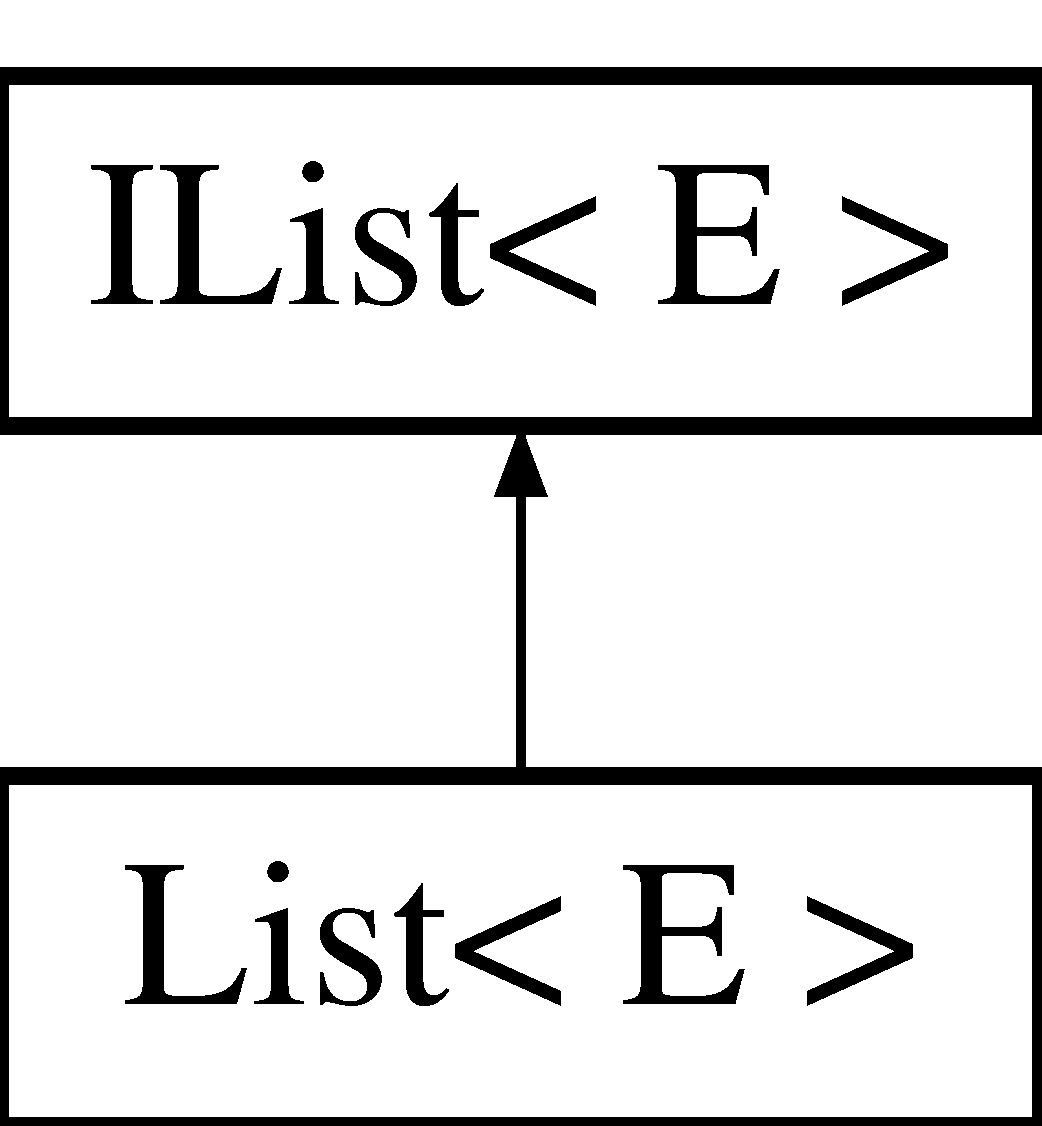
\includegraphics[height=2.000000cm]{classList}
\end{center}
\end{figure}
\subsection*{Public Member Functions}
\begin{DoxyCompactItemize}
\item 
void \hyperlink{classList_a40dfa61150de7310d69001c697598b04}{addi} (E)
\item 
void \hyperlink{classList_a2a130b7bc38cd968136f1f847e42d0cc}{add} (E)
\item 
bool \hyperlink{classList_a530267346ebec244900c162de6f467e1}{add} (E, int)
\item 
bool \hyperlink{classList_a46cec78299d3e23469276adf46adf9c1}{remove} (int)
\item 
void \hyperlink{classList_ac8b31be96806bd56f655436629ac2e7a}{set} (int, E)
\item 
E \hyperlink{classList_ab081a52d7a62aa6c5550ff9762f9427f}{get} (int)
\item 
\hyperlink{classSimpleIterator}{Simple\-Iterator}$<$ E $>$ $\ast$ \hyperlink{classList_accb5fe71cb60ba7bf0ccab362b1f87cb}{get\-Iterator} ()
\item 
\hypertarget{classList_ad2201bc77b15291f215523ecc96705dc}{void {\bfseries print} () const }\label{classList_ad2201bc77b15291f215523ecc96705dc}

\end{DoxyCompactItemize}
\subsection*{Protected Attributes}
\begin{DoxyCompactItemize}
\item 
\hyperlink{classNode}{Node}$<$ E $>$ $\ast$ \hyperlink{classList_ae3829eca87a5040cca1ae9e0dc40b768}{head}
\item 
\hyperlink{classNode}{Node}$<$ E $>$ $\ast$ \hyperlink{classList_a6008ce8286d474397d0ce5847f819783}{tail}
\end{DoxyCompactItemize}


\subsection{Member Function Documentation}
\hypertarget{classList_a2a130b7bc38cd968136f1f847e42d0cc}{\index{List@{List}!add@{add}}
\index{add@{add}!List@{List}}
\subsubsection[{add}]{\setlength{\rightskip}{0pt plus 5cm}template$<$class E $>$ void {\bf List}$<$ E $>$\-::add (
\begin{DoxyParamCaption}
\item[{E}]{data}
\end{DoxyParamCaption}
)\hspace{0.3cm}{\ttfamily [virtual]}}}\label{classList_a2a130b7bc38cd968136f1f847e42d0cc}

\begin{DoxyParams}{Parameters}
{\em E} & \\
\hline
{\em data} & \\
\hline
\end{DoxyParams}


Implements \hyperlink{classIList_a27500caa3d9da05aa6437d5ff56b09e2}{I\-List$<$ E $>$}.

\hypertarget{classList_a530267346ebec244900c162de6f467e1}{\index{List@{List}!add@{add}}
\index{add@{add}!List@{List}}
\subsubsection[{add}]{\setlength{\rightskip}{0pt plus 5cm}template$<$class E $>$ bool {\bf List}$<$ E $>$\-::add (
\begin{DoxyParamCaption}
\item[{E}]{data, }
\item[{int}]{index}
\end{DoxyParamCaption}
)\hspace{0.3cm}{\ttfamily [virtual]}}}\label{classList_a530267346ebec244900c162de6f467e1}

\begin{DoxyParams}{Parameters}
{\em E} & \\
\hline
{\em int} & \\
\hline
\end{DoxyParams}
\begin{DoxyReturn}{Returns}
bool
\end{DoxyReturn}

\begin{DoxyParams}{Parameters}
{\em data} & \\
\hline
{\em index} & \\
\hline
\end{DoxyParams}
\begin{DoxyReturn}{Returns}
bool List$<$\-E$>$ 
\end{DoxyReturn}


Implements \hyperlink{classIList_a70140dbc9de2b9f6e5ffd2212d5ea8b0}{I\-List$<$ E $>$}.

\hypertarget{classList_a40dfa61150de7310d69001c697598b04}{\index{List@{List}!addi@{addi}}
\index{addi@{addi}!List@{List}}
\subsubsection[{addi}]{\setlength{\rightskip}{0pt plus 5cm}template$<$class E $>$ void {\bf List}$<$ E $>$\-::addi (
\begin{DoxyParamCaption}
\item[{E}]{data}
\end{DoxyParamCaption}
)\hspace{0.3cm}{\ttfamily [virtual]}}}\label{classList_a40dfa61150de7310d69001c697598b04}

\begin{DoxyParams}{Parameters}
{\em E} & \\
\hline
{\em data} & \\
\hline
\end{DoxyParams}


Implements \hyperlink{classIList_af202dc9e748ee32238d80e57dfbcae20}{I\-List$<$ E $>$}.

\hypertarget{classList_ab081a52d7a62aa6c5550ff9762f9427f}{\index{List@{List}!get@{get}}
\index{get@{get}!List@{List}}
\subsubsection[{get}]{\setlength{\rightskip}{0pt plus 5cm}template$<$class E $>$ E {\bf List}$<$ E $>$\-::get (
\begin{DoxyParamCaption}
\item[{int}]{index}
\end{DoxyParamCaption}
)\hspace{0.3cm}{\ttfamily [virtual]}}}\label{classList_ab081a52d7a62aa6c5550ff9762f9427f}

\begin{DoxyParams}{Parameters}
{\em int} & \\
\hline
\end{DoxyParams}
\begin{DoxyReturn}{Returns}
E
\end{DoxyReturn}

\begin{DoxyParams}{Parameters}
{\em index} & \\
\hline
\end{DoxyParams}
\begin{DoxyReturn}{Returns}
E List$<$\-E$>$ 
\end{DoxyReturn}


Implements \hyperlink{classIList_a60570f7ee0e7474d01b2f364bad996a0}{I\-List$<$ E $>$}.

\hypertarget{classList_accb5fe71cb60ba7bf0ccab362b1f87cb}{\index{List@{List}!get\-Iterator@{get\-Iterator}}
\index{get\-Iterator@{get\-Iterator}!List@{List}}
\subsubsection[{get\-Iterator}]{\setlength{\rightskip}{0pt plus 5cm}template$<$class E $>$ {\bf Simple\-Iterator}$<$ E $>$ $\ast$ {\bf List}$<$ E $>$\-::get\-Iterator (
\begin{DoxyParamCaption}
{}
\end{DoxyParamCaption}
)}}\label{classList_accb5fe71cb60ba7bf0ccab362b1f87cb}
\begin{DoxyReturn}{Returns}
Simple\-Iterator$<$\-E$>$

Simple\-Iterator$<$\-E$>$ $\ast$\-List$<$\-E$>$ 
\end{DoxyReturn}
\hypertarget{classList_a46cec78299d3e23469276adf46adf9c1}{\index{List@{List}!remove@{remove}}
\index{remove@{remove}!List@{List}}
\subsubsection[{remove}]{\setlength{\rightskip}{0pt plus 5cm}template$<$class E $>$ bool {\bf List}$<$ E $>$\-::remove (
\begin{DoxyParamCaption}
\item[{int}]{index}
\end{DoxyParamCaption}
)\hspace{0.3cm}{\ttfamily [virtual]}}}\label{classList_a46cec78299d3e23469276adf46adf9c1}

\begin{DoxyParams}{Parameters}
{\em int} & \\
\hline
\end{DoxyParams}
\begin{DoxyReturn}{Returns}
bool
\end{DoxyReturn}

\begin{DoxyParams}{Parameters}
{\em index} & \\
\hline
\end{DoxyParams}
\begin{DoxyReturn}{Returns}
bool List$<$\-E$>$ 
\end{DoxyReturn}


Implements \hyperlink{classIList_a9bf7d737252dfbd4c9a5d7be36ea4231}{I\-List$<$ E $>$}.

\hypertarget{classList_ac8b31be96806bd56f655436629ac2e7a}{\index{List@{List}!set@{set}}
\index{set@{set}!List@{List}}
\subsubsection[{set}]{\setlength{\rightskip}{0pt plus 5cm}template$<$class E $>$ void {\bf List}$<$ E $>$\-::set (
\begin{DoxyParamCaption}
\item[{int}]{index, }
\item[{E}]{data}
\end{DoxyParamCaption}
)\hspace{0.3cm}{\ttfamily [virtual]}}}\label{classList_ac8b31be96806bd56f655436629ac2e7a}

\begin{DoxyParams}{Parameters}
{\em int} & \\
\hline
{\em E} & \\
\hline
{\em index} & \\
\hline
{\em data} & \\
\hline
\end{DoxyParams}


Implements \hyperlink{classIList_a119ed658d2804aec0b9fef9325c03073}{I\-List$<$ E $>$}.



\subsection{Member Data Documentation}
\hypertarget{classList_ae3829eca87a5040cca1ae9e0dc40b768}{\index{List@{List}!head@{head}}
\index{head@{head}!List@{List}}
\subsubsection[{head}]{\setlength{\rightskip}{0pt plus 5cm}template$<$class E $>$ {\bf Node}$<$E$>$$\ast$ {\bf List}$<$ E $>$\-::head\hspace{0.3cm}{\ttfamily [protected]}}}\label{classList_ae3829eca87a5040cca1ae9e0dc40b768}
T\-O\-D\-O \hypertarget{classList_a6008ce8286d474397d0ce5847f819783}{\index{List@{List}!tail@{tail}}
\index{tail@{tail}!List@{List}}
\subsubsection[{tail}]{\setlength{\rightskip}{0pt plus 5cm}template$<$class E $>$ {\bf Node}$<$E$>$$\ast$ {\bf List}$<$ E $>$\-::tail\hspace{0.3cm}{\ttfamily [protected]}}}\label{classList_a6008ce8286d474397d0ce5847f819783}
T\-O\-D\-O 

The documentation for this class was generated from the following file\-:\begin{DoxyCompactItemize}
\item 
list/List.\-hpp\end{DoxyCompactItemize}

\hypertarget{classNode}{\section{Referencia de la plantilla de la Clase Node$<$ E $>$}
\label{classNode}\index{Node$<$ E $>$@{Node$<$ E $>$}}
}


Es la parte elemental de una lista simple.  




{\ttfamily \#include $<$Node.\-h$>$}

\subsection*{Métodos públicos}
\begin{DoxyCompactItemize}
\item 
\hyperlink{classNode_a74d41f93c30d8c3036d24894f0e4314e}{Node} (E)
\begin{DoxyCompactList}\small\item\em Constructor del Nodo, el next se setea como un puntero nulo para evitar punteros colgados. \end{DoxyCompactList}\item 
\hyperlink{classNode_adc1b4c81c3fb6d0580f138650629a41e}{Node} (E data, \hyperlink{classNode}{Node}$<$ E $>$ $\ast$next)
\begin{DoxyCompactList}\small\item\em Constructor del Nodo. \end{DoxyCompactList}\item 
void \hyperlink{classNode_ae13418a552fa36eddbaa5dfb767aa664}{set\-Data} (E)
\begin{DoxyCompactList}\small\item\em Setea el dato contenido en el nodo. \end{DoxyCompactList}\item 
E \hyperlink{classNode_a02a4e5126542aaa1a2150932cfa2b8ce}{get\-Data} () const 
\begin{DoxyCompactList}\small\item\em Obtiene el dato contenido en el nodo. \end{DoxyCompactList}\item 
\hypertarget{classNode_adec417c9f6f7d2cbd0fc7a72508e9c3d}{E \& {\bfseries get\-Reference\-Data} ()}\label{classNode_adec417c9f6f7d2cbd0fc7a72508e9c3d}

\item 
void \hyperlink{classNode_a2ce12b4f2605972720e1c56fe80014a0}{set\-Next} (\hyperlink{classNode}{Node}$<$ E $>$ $\ast$)
\begin{DoxyCompactList}\small\item\em Setea el puntero del nodo siguiente. \end{DoxyCompactList}\item 
\hyperlink{classNode}{Node}$<$ E $>$ $\ast$ \hyperlink{classNode_aeb063e5172867e988550ab7d6c280db7}{get\-Next} () const 
\begin{DoxyCompactList}\small\item\em Obtiene el nodo siguiente. \end{DoxyCompactList}\item 
\hypertarget{classNode_af907944256d9fca41c6a1c783a3a6536}{virtual \hyperlink{classNode_af907944256d9fca41c6a1c783a3a6536}{$\sim$\-Node} ()}\label{classNode_af907944256d9fca41c6a1c783a3a6536}

\begin{DoxyCompactList}\small\item\em Liberador de memoria. \end{DoxyCompactList}\end{DoxyCompactItemize}


\subsection{Descripción detallada}
\subsubsection*{template$<$class E$>$class Node$<$ E $>$}

Es la parte elemental de una lista simple. 

\subsection{Documentación del constructor y destructor}
\hypertarget{classNode_a74d41f93c30d8c3036d24894f0e4314e}{\index{Node@{Node}!Node@{Node}}
\index{Node@{Node}!Node@{Node}}
\subsubsection[{Node}]{\setlength{\rightskip}{0pt plus 5cm}template$<$class E $>$ {\bf Node}$<$ E $>$\-::{\bf Node} (
\begin{DoxyParamCaption}
\item[{E}]{data}
\end{DoxyParamCaption}
)}}\label{classNode_a74d41f93c30d8c3036d24894f0e4314e}


Constructor del Nodo, el next se setea como un puntero nulo para evitar punteros colgados. 


\begin{DoxyParams}{Parámetros}
{\em data} & el dato que contrendra el nodo \\
\hline
\end{DoxyParams}
\hypertarget{classNode_adc1b4c81c3fb6d0580f138650629a41e}{\index{Node@{Node}!Node@{Node}}
\index{Node@{Node}!Node@{Node}}
\subsubsection[{Node}]{\setlength{\rightskip}{0pt plus 5cm}template$<$class E $>$ {\bf Node}$<$ E $>$\-::{\bf Node} (
\begin{DoxyParamCaption}
\item[{E}]{data, }
\item[{{\bf Node}$<$ E $>$ $\ast$}]{next}
\end{DoxyParamCaption}
)}}\label{classNode_adc1b4c81c3fb6d0580f138650629a41e}


Constructor del Nodo. 


\begin{DoxyParams}{Parámetros}
{\em data} & el dato que contendra el dato \\
\hline
{\em next} & el puntero al nodo siguiente \\
\hline
\end{DoxyParams}


\subsection{Documentación de las funciones miembro}
\hypertarget{classNode_a02a4e5126542aaa1a2150932cfa2b8ce}{\index{Node@{Node}!get\-Data@{get\-Data}}
\index{get\-Data@{get\-Data}!Node@{Node}}
\subsubsection[{get\-Data}]{\setlength{\rightskip}{0pt plus 5cm}template$<$class E $>$ E {\bf Node}$<$ E $>$\-::get\-Data (
\begin{DoxyParamCaption}
{}
\end{DoxyParamCaption}
) const}}\label{classNode_a02a4e5126542aaa1a2150932cfa2b8ce}


Obtiene el dato contenido en el nodo. 

\begin{DoxyReturn}{Devuelve}
E el dato contenido 
\end{DoxyReturn}
\hypertarget{classNode_aeb063e5172867e988550ab7d6c280db7}{\index{Node@{Node}!get\-Next@{get\-Next}}
\index{get\-Next@{get\-Next}!Node@{Node}}
\subsubsection[{get\-Next}]{\setlength{\rightskip}{0pt plus 5cm}template$<$class E $>$ {\bf Node}$<$ E $>$ $\ast$ {\bf Node}$<$ E $>$\-::get\-Next (
\begin{DoxyParamCaption}
{}
\end{DoxyParamCaption}
) const}}\label{classNode_aeb063e5172867e988550ab7d6c280db7}


Obtiene el nodo siguiente. 

\begin{DoxyReturn}{Devuelve}
Double\-Node$<$\-E$>$ el nodo siguiente 
\end{DoxyReturn}
\hypertarget{classNode_ae13418a552fa36eddbaa5dfb767aa664}{\index{Node@{Node}!set\-Data@{set\-Data}}
\index{set\-Data@{set\-Data}!Node@{Node}}
\subsubsection[{set\-Data}]{\setlength{\rightskip}{0pt plus 5cm}template$<$class E $>$ void {\bf Node}$<$ E $>$\-::set\-Data (
\begin{DoxyParamCaption}
\item[{E}]{data}
\end{DoxyParamCaption}
)}}\label{classNode_ae13418a552fa36eddbaa5dfb767aa664}


Setea el dato contenido en el nodo. 


\begin{DoxyParams}{Parámetros}
{\em data} & el dato nuevo \\
\hline
\end{DoxyParams}
\hypertarget{classNode_a2ce12b4f2605972720e1c56fe80014a0}{\index{Node@{Node}!set\-Next@{set\-Next}}
\index{set\-Next@{set\-Next}!Node@{Node}}
\subsubsection[{set\-Next}]{\setlength{\rightskip}{0pt plus 5cm}template$<$class E $>$ void {\bf Node}$<$ E $>$\-::set\-Next (
\begin{DoxyParamCaption}
\item[{{\bf Node}$<$ E $>$ $\ast$}]{next}
\end{DoxyParamCaption}
)}}\label{classNode_a2ce12b4f2605972720e1c56fe80014a0}


Setea el puntero del nodo siguiente. 


\begin{DoxyParams}{Parámetros}
{\em next} & el nuevo nodo que representa el nodo siguiente \\
\hline
\end{DoxyParams}


La documentación para esta clase fue generada a partir del siguiente fichero\-:\begin{DoxyCompactItemize}
\item 
list/Node.\-h\end{DoxyCompactItemize}

\hypertarget{classQueue}{\section{Queue$<$ E $>$ Class Template Reference}
\label{classQueue}\index{Queue$<$ E $>$@{Queue$<$ E $>$}}
}
\subsection*{Public Member Functions}
\begin{DoxyCompactItemize}
\item 
\hypertarget{classQueue_ab09891e54b51dc677ee6efb350687ae4}{\hyperlink{classQueue_ab09891e54b51dc677ee6efb350687ae4}{Queue} ()}\label{classQueue_ab09891e54b51dc677ee6efb350687ae4}

\begin{DoxyCompactList}\small\item\em Metodo constructor. \end{DoxyCompactList}\item 
void \hyperlink{classQueue_ad751a5ab9f313291a85455542b12a184}{enqueue} (E data)
\begin{DoxyCompactList}\small\item\em Agrega de ultimo el dato a encolar. \end{DoxyCompactList}\item 
E \hyperlink{classQueue_ac2b0f94e80e6df3002d284e38bdc117b}{dequeue} ()
\begin{DoxyCompactList}\small\item\em Elimina el primer nodo encolado. \end{DoxyCompactList}\item 
bool \hyperlink{classQueue_ab652261bbb405ecc84a80ff5d7139de7}{is\-Empty} ()
\begin{DoxyCompactList}\small\item\em Retorna verdadero si la pila esta vacia, de lo contrario retorna falso. \end{DoxyCompactList}\end{DoxyCompactItemize}


\subsection{Member Function Documentation}
\hypertarget{classQueue_ac2b0f94e80e6df3002d284e38bdc117b}{\index{Queue@{Queue}!dequeue@{dequeue}}
\index{dequeue@{dequeue}!Queue@{Queue}}
\subsubsection[{dequeue}]{\setlength{\rightskip}{0pt plus 5cm}template$<$class E $>$ E {\bf Queue}$<$ E $>$\-::dequeue (
\begin{DoxyParamCaption}
{}
\end{DoxyParamCaption}
)}}\label{classQueue_ac2b0f94e80e6df3002d284e38bdc117b}


Elimina el primer nodo encolado. 

\begin{DoxyReturn}{Returns}
E el dato desencolado 
\end{DoxyReturn}
\hypertarget{classQueue_ad751a5ab9f313291a85455542b12a184}{\index{Queue@{Queue}!enqueue@{enqueue}}
\index{enqueue@{enqueue}!Queue@{Queue}}
\subsubsection[{enqueue}]{\setlength{\rightskip}{0pt plus 5cm}template$<$class E $>$ void {\bf Queue}$<$ E $>$\-::enqueue (
\begin{DoxyParamCaption}
\item[{E}]{data}
\end{DoxyParamCaption}
)}}\label{classQueue_ad751a5ab9f313291a85455542b12a184}


Agrega de ultimo el dato a encolar. 


\begin{DoxyParams}{Parameters}
{\em data} & el dato a encolar \\
\hline
\end{DoxyParams}
\hypertarget{classQueue_ab652261bbb405ecc84a80ff5d7139de7}{\index{Queue@{Queue}!is\-Empty@{is\-Empty}}
\index{is\-Empty@{is\-Empty}!Queue@{Queue}}
\subsubsection[{is\-Empty}]{\setlength{\rightskip}{0pt plus 5cm}template$<$class E $>$ {\bf Queue}$<$ E $>$\-::is\-Empty (
\begin{DoxyParamCaption}
{}
\end{DoxyParamCaption}
)}}\label{classQueue_ab652261bbb405ecc84a80ff5d7139de7}


Retorna verdadero si la pila esta vacia, de lo contrario retorna falso. 

\begin{DoxyReturn}{Returns}
bool 
\end{DoxyReturn}


The documentation for this class was generated from the following file\-:\begin{DoxyCompactItemize}
\item 
control\-Structure/Queue.\-h\end{DoxyCompactItemize}

\hypertarget{classSimpleIterator}{\section{Referencia de la plantilla de la Clase Simple\-Iterator$<$ E $>$}
\label{classSimpleIterator}\index{Simple\-Iterator$<$ E $>$@{Simple\-Iterator$<$ E $>$}}
}


Esta clase es un iterador de las listas simples, ademas la actualizacion de la lista N\-O actualiza el iterador, por lo que el iterador es momentaneo. Es similar a una fotografia de una lista que no ha sido alterada si la lista se altera usando un iterador puede que el iterador falle. Por lo que es recomendable que la lista no se actualice mientras se usa un iterador.  




{\ttfamily \#include $<$Simple\-Iterator.\-h$>$}



Herencias \hyperlink{classIIterator}{I\-Iterator$<$ E $>$}.

\subsection*{Métodos públicos}
\begin{DoxyCompactItemize}
\item 
E \hyperlink{classSimpleIterator_ab01032dba9ff4f1a1c47af3082b717d5}{get\-Next} ()
\begin{DoxyCompactList}\small\item\em Obtiene el dato actual y actualiza al nodo siguiente. \end{DoxyCompactList}\item 
E \hyperlink{classSimpleIterator_ac9460c98985a20f781f351c85b8a3ba2}{get\-Current} () const 
\begin{DoxyCompactList}\small\item\em Obtiene el dato actual. \end{DoxyCompactList}\item 
bool \hyperlink{classSimpleIterator_ab946b3d707e32d4d53f15af201ea2113}{has\-Next} () const 
\begin{DoxyCompactList}\small\item\em Verifica si tiene siguiente. \end{DoxyCompactList}\item 
\hypertarget{classSimpleIterator_a02203109d263581340152408ebb120a2}{virtual \hyperlink{classSimpleIterator_a02203109d263581340152408ebb120a2}{$\sim$\-Simple\-Iterator} ()}\label{classSimpleIterator_a02203109d263581340152408ebb120a2}

\begin{DoxyCompactList}\small\item\em Liberador de memoria. \end{DoxyCompactList}\end{DoxyCompactItemize}
\subsection*{Atributos protegidos}
\begin{DoxyCompactItemize}
\item 
\hypertarget{classSimpleIterator_a0403100ab86dba958115cea4147508a7}{\hyperlink{classNode}{Node}$<$ E $>$ $\ast$ {\bfseries head}}\label{classSimpleIterator_a0403100ab86dba958115cea4147508a7}

\item 
\hypertarget{classSimpleIterator_a9bfb7d6c12bc1e8031b5c0869026415a}{\hyperlink{classNode}{Node}$<$ E $>$ $\ast$ {\bfseries tail}}\label{classSimpleIterator_a9bfb7d6c12bc1e8031b5c0869026415a}

\item 
\hyperlink{classNode}{Node}$<$ E $>$ $\ast$ \hyperlink{classSimpleIterator_a7777fefe265a5067ec9319d8c1a3e278}{current}
\end{DoxyCompactItemize}
\subsection*{Amigas}
\begin{DoxyCompactItemize}
\item 
\hypertarget{classSimpleIterator_a8740adf5dfdafdc64940ab42ed663bd2}{{\footnotesize template$<$class T $>$ }\\class {\bfseries List}}\label{classSimpleIterator_a8740adf5dfdafdc64940ab42ed663bd2}

\item 
\hypertarget{classSimpleIterator_ade98163865dd2cf1343ae0a4dbba6b29}{{\footnotesize template$<$class M $>$ }\\class {\bfseries Circular\-List}}\label{classSimpleIterator_ade98163865dd2cf1343ae0a4dbba6b29}

\end{DoxyCompactItemize}


\subsection{Descripción detallada}
\subsubsection*{template$<$class E$>$class Simple\-Iterator$<$ E $>$}

Esta clase es un iterador de las listas simples, ademas la actualizacion de la lista N\-O actualiza el iterador, por lo que el iterador es momentaneo. Es similar a una fotografia de una lista que no ha sido alterada si la lista se altera usando un iterador puede que el iterador falle. Por lo que es recomendable que la lista no se actualice mientras se usa un iterador. 

\subsection{Documentación de las funciones miembro}
\hypertarget{classSimpleIterator_ac9460c98985a20f781f351c85b8a3ba2}{\index{Simple\-Iterator@{Simple\-Iterator}!get\-Current@{get\-Current}}
\index{get\-Current@{get\-Current}!SimpleIterator@{Simple\-Iterator}}
\subsubsection[{get\-Current}]{\setlength{\rightskip}{0pt plus 5cm}template$<$class E $>$ E {\bf Simple\-Iterator}$<$ E $>$\-::get\-Current (
\begin{DoxyParamCaption}
{}
\end{DoxyParamCaption}
) const\hspace{0.3cm}{\ttfamily [virtual]}}}\label{classSimpleIterator_ac9460c98985a20f781f351c85b8a3ba2}


Obtiene el dato actual. 

\begin{DoxyReturn}{Devuelve}
E el dato actual 
\end{DoxyReturn}

\begin{DoxyExceptions}{Excepciones}
{\em donthavenext} & si el dato actual es nulo \\
\hline
\end{DoxyExceptions}


Implementa \hyperlink{classIIterator_a50f55ce1381378aad2c93f16c9b60822}{I\-Iterator$<$ E $>$}.

\hypertarget{classSimpleIterator_ab01032dba9ff4f1a1c47af3082b717d5}{\index{Simple\-Iterator@{Simple\-Iterator}!get\-Next@{get\-Next}}
\index{get\-Next@{get\-Next}!SimpleIterator@{Simple\-Iterator}}
\subsubsection[{get\-Next}]{\setlength{\rightskip}{0pt plus 5cm}template$<$class E $>$ E {\bf Simple\-Iterator}$<$ E $>$\-::get\-Next (
\begin{DoxyParamCaption}
{}
\end{DoxyParamCaption}
)\hspace{0.3cm}{\ttfamily [virtual]}}}\label{classSimpleIterator_ab01032dba9ff4f1a1c47af3082b717d5}


Obtiene el dato actual y actualiza al nodo siguiente. 

\begin{DoxyReturn}{Devuelve}
E el dato actual 
\end{DoxyReturn}

\begin{DoxyExceptions}{Excepciones}
{\em donthavenext} & si el dato actual es nulo \\
\hline
\end{DoxyExceptions}


Implementa \hyperlink{classIIterator_ab1b13434e4fac20c74262dee51d1e870}{I\-Iterator$<$ E $>$}.

\hypertarget{classSimpleIterator_ab946b3d707e32d4d53f15af201ea2113}{\index{Simple\-Iterator@{Simple\-Iterator}!has\-Next@{has\-Next}}
\index{has\-Next@{has\-Next}!SimpleIterator@{Simple\-Iterator}}
\subsubsection[{has\-Next}]{\setlength{\rightskip}{0pt plus 5cm}template$<$class E $>$ bool {\bf Simple\-Iterator}$<$ E $>$\-::has\-Next (
\begin{DoxyParamCaption}
{}
\end{DoxyParamCaption}
) const\hspace{0.3cm}{\ttfamily [virtual]}}}\label{classSimpleIterator_ab946b3d707e32d4d53f15af201ea2113}


Verifica si tiene siguiente. 

\begin{DoxyReturn}{Devuelve}
true si tiene siguiente, false si no lo tiene 
\end{DoxyReturn}

\begin{DoxyExceptions}{Excepciones}
{\em donthavenext} & si el dato actual es nulo \\
\hline
\end{DoxyExceptions}


Implementa \hyperlink{classIIterator_a8a73f0fb41a66fe98e5e636378759196}{I\-Iterator$<$ E $>$}.



\subsection{Documentación de los datos miembro}
\hypertarget{classSimpleIterator_a7777fefe265a5067ec9319d8c1a3e278}{\index{Simple\-Iterator@{Simple\-Iterator}!current@{current}}
\index{current@{current}!SimpleIterator@{Simple\-Iterator}}
\subsubsection[{current}]{\setlength{\rightskip}{0pt plus 5cm}template$<$class E$>$ {\bf Node}$<$E$>$ $\ast$ {\bf Simple\-Iterator}$<$ E $>$\-::current\hspace{0.3cm}{\ttfamily [protected]}}}\label{classSimpleIterator_a7777fefe265a5067ec9319d8c1a3e278}
T\-O\-D\-O 

La documentación para esta clase fue generada a partir del siguiente fichero\-:\begin{DoxyCompactItemize}
\item 
list/Simple\-Iterator.\-h\end{DoxyCompactItemize}

\hypertarget{classStack}{\section{Stack$<$ E $>$ Class Template Reference}
\label{classStack}\index{Stack$<$ E $>$@{Stack$<$ E $>$}}
}
\subsection*{Public Member Functions}
\begin{DoxyCompactItemize}
\item 
\hypertarget{classStack_a561be1726ac9649a9ee3f80a4ca8e4b5}{\hyperlink{classStack_a561be1726ac9649a9ee3f80a4ca8e4b5}{Stack} ()}\label{classStack_a561be1726ac9649a9ee3f80a4ca8e4b5}

\begin{DoxyCompactList}\small\item\em Metodo constructor. \end{DoxyCompactList}\item 
void \hyperlink{classStack_af71e3e142fba5bb861b66b4882289b31}{push} (E)
\begin{DoxyCompactList}\small\item\em Agrega el dato a la cima de la pila. \end{DoxyCompactList}\item 
E \hyperlink{classStack_a5ba7a4c8eec39757e28f95da49f06d52}{pop} ()
\begin{DoxyCompactList}\small\item\em Elimina de la pila y retorna el dato de la cima de la pila. En caso de que la pila este vacia se produce un error. \end{DoxyCompactList}\item 
E \hyperlink{classStack_a19a17240bf7045cf6a3a9497e1091433}{peek} () const 
\begin{DoxyCompactList}\small\item\em Revisa el dato en la cima de la pila. En caso de que la pila este vacia se produce un error. \end{DoxyCompactList}\item 
bool \hyperlink{classStack_a0ce2804f35c0c8cfb999535f35fa438b}{is\-Empty} ()
\begin{DoxyCompactList}\small\item\em Retorna verdadero si la pila esta vacia de lo contrario retorna falso. \end{DoxyCompactList}\item 
\hypertarget{classStack_ad08e4c32f07b8d967913f8b1a45f8620}{virtual \hyperlink{classStack_ad08e4c32f07b8d967913f8b1a45f8620}{$\sim$\-Stack} ()}\label{classStack_ad08e4c32f07b8d967913f8b1a45f8620}

\begin{DoxyCompactList}\small\item\em Metodo destructor, borra todos los elementos de la pila. \end{DoxyCompactList}\end{DoxyCompactItemize}


\subsection{Member Function Documentation}
\hypertarget{classStack_a0ce2804f35c0c8cfb999535f35fa438b}{\index{Stack@{Stack}!is\-Empty@{is\-Empty}}
\index{is\-Empty@{is\-Empty}!Stack@{Stack}}
\subsubsection[{is\-Empty}]{\setlength{\rightskip}{0pt plus 5cm}template$<$class E $>$ bool {\bf Stack}$<$ E $>$\-::is\-Empty (
\begin{DoxyParamCaption}
{}
\end{DoxyParamCaption}
)}}\label{classStack_a0ce2804f35c0c8cfb999535f35fa438b}


Retorna verdadero si la pila esta vacia de lo contrario retorna falso. 

\begin{DoxyReturn}{Returns}
bool el valor de verdad de la frase ¿esta vacia la pila? 
\end{DoxyReturn}
\hypertarget{classStack_a19a17240bf7045cf6a3a9497e1091433}{\index{Stack@{Stack}!peek@{peek}}
\index{peek@{peek}!Stack@{Stack}}
\subsubsection[{peek}]{\setlength{\rightskip}{0pt plus 5cm}template$<$class E $>$ E {\bf Stack}$<$ E $>$\-::peek (
\begin{DoxyParamCaption}
{}
\end{DoxyParamCaption}
) const}}\label{classStack_a19a17240bf7045cf6a3a9497e1091433}


Revisa el dato en la cima de la pila. En caso de que la pila este vacia se produce un error. 

\begin{DoxyReturn}{Returns}
E el dato de la cima 
\end{DoxyReturn}
\hypertarget{classStack_a5ba7a4c8eec39757e28f95da49f06d52}{\index{Stack@{Stack}!pop@{pop}}
\index{pop@{pop}!Stack@{Stack}}
\subsubsection[{pop}]{\setlength{\rightskip}{0pt plus 5cm}template$<$class E $>$ E {\bf Stack}$<$ E $>$\-::pop (
\begin{DoxyParamCaption}
{}
\end{DoxyParamCaption}
)}}\label{classStack_a5ba7a4c8eec39757e28f95da49f06d52}


Elimina de la pila y retorna el dato de la cima de la pila. En caso de que la pila este vacia se produce un error. 

\begin{DoxyReturn}{Returns}
E el dato en la cima. 
\end{DoxyReturn}
\hypertarget{classStack_af71e3e142fba5bb861b66b4882289b31}{\index{Stack@{Stack}!push@{push}}
\index{push@{push}!Stack@{Stack}}
\subsubsection[{push}]{\setlength{\rightskip}{0pt plus 5cm}template$<$class E $>$ void {\bf Stack}$<$ E $>$\-::push (
\begin{DoxyParamCaption}
\item[{E}]{data}
\end{DoxyParamCaption}
)}}\label{classStack_af71e3e142fba5bb861b66b4882289b31}


Agrega el dato a la cima de la pila. 


\begin{DoxyParams}{Parameters}
{\em E} & el dato a agregar. \\
\hline
\end{DoxyParams}


The documentation for this class was generated from the following file\-:\begin{DoxyCompactItemize}
\item 
control\-Structure/Stack.\-h\end{DoxyCompactItemize}

%--- End generated contents ---

% Index
\newpage
\phantomsection
\addcontentsline{toc}{chapter}{Index}
\printindex

\end{document}
